\section{Results}
\label{sec:results}
This section deals with the results of the electrical characterisation of the neutron-irradiated HGCAL silicon pad sensor prototypes. 
\ref{subsec:leakagecurrents} focuses on the discussion of leakage currents (IV) whereas \ref{subsec:Udep} addresses the findings of the capacitance and depletion voltage assessments. 
The presentation of the results is complemented in \ref{subsec:discussion} with a discussion on the limitations in their interpretability and on the drawn conclusion.

\subsection{Leakage Current}
\label{subsec:leakagecurrents}
\begin{figure}
	\captionsetup[subfigure]{aboveskip=-1pt,belowskip=-1pt}
	\centering
	\begin{subfigure}[b]{0.49\textwidth}
		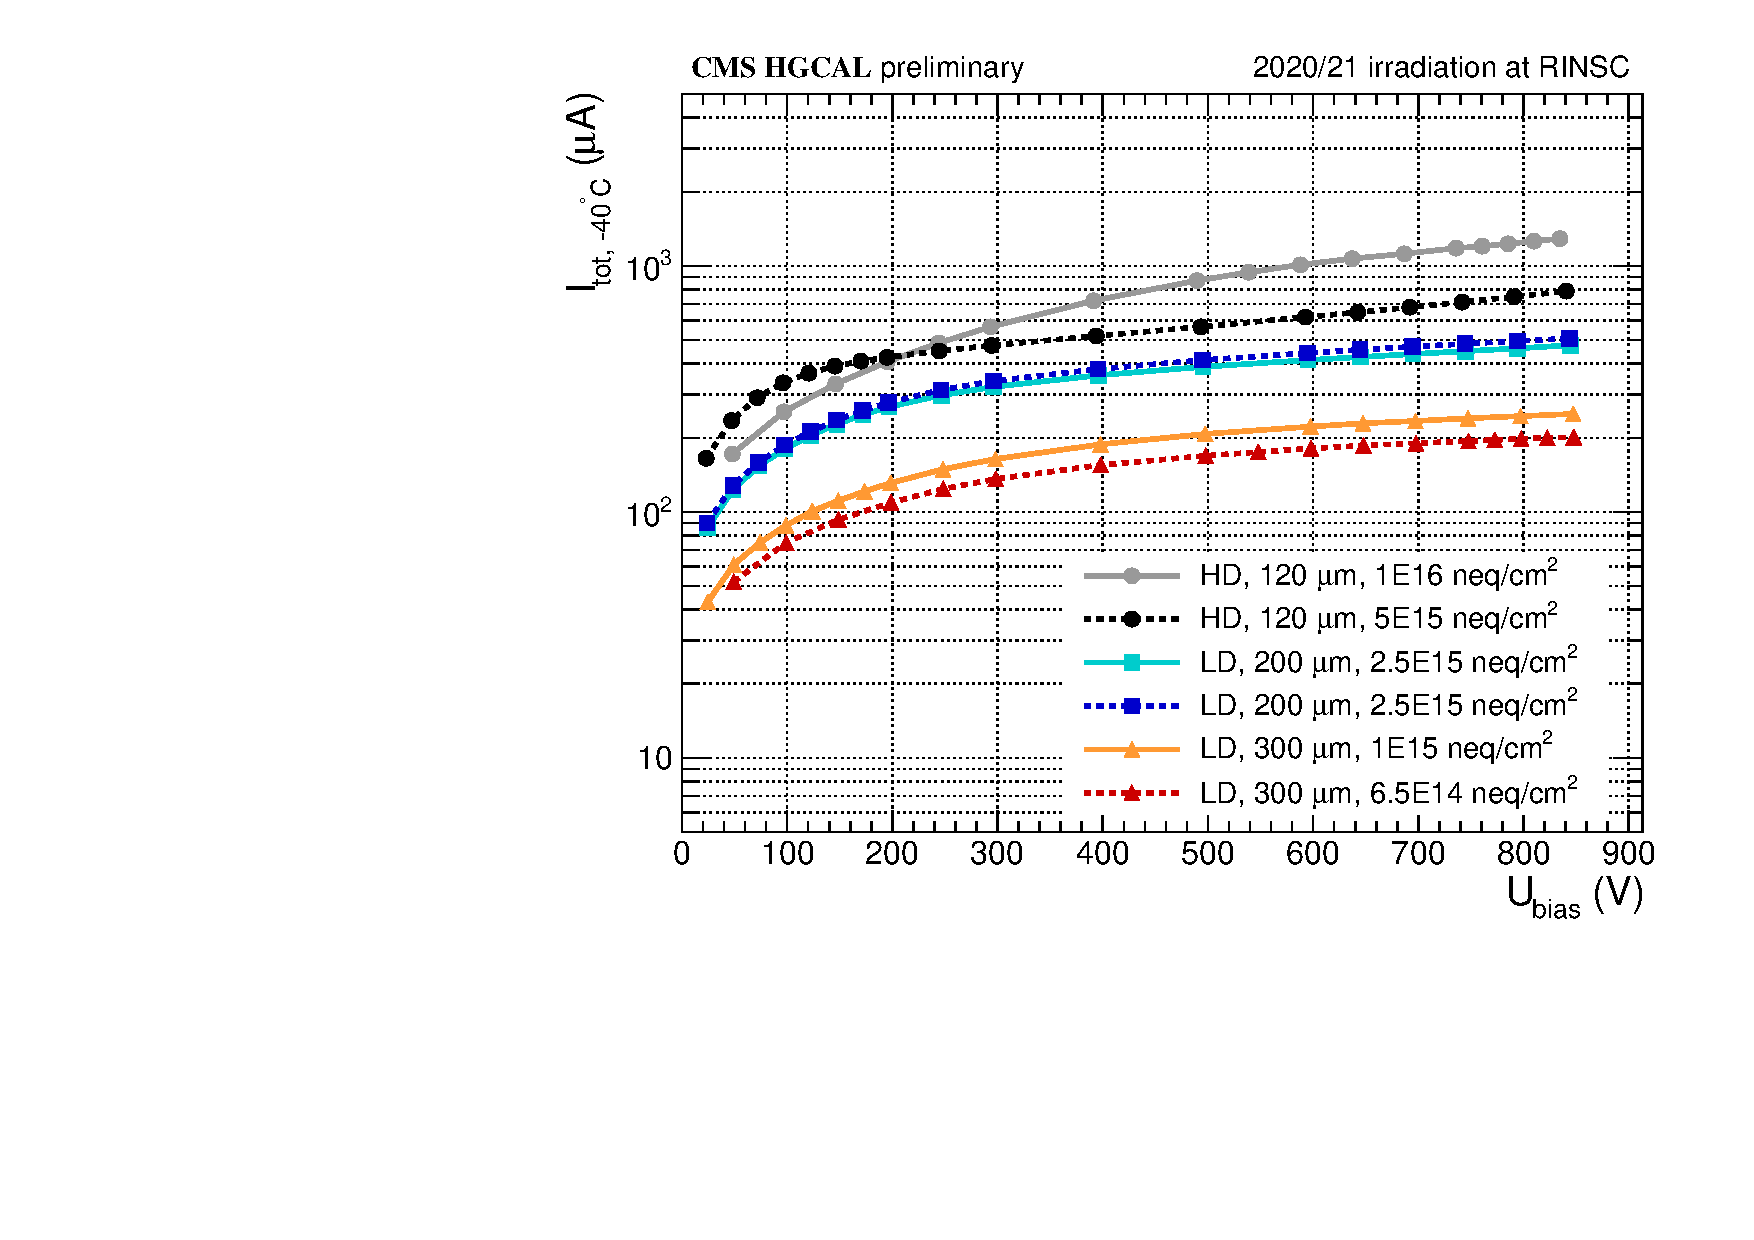
\includegraphics[width=0.999\textwidth]{plots/total_iv/total_current_IV.pdf}
		\subcaption{
		}
		\label{plot:tot_IV_good}
    \end{subfigure}
    \hfill
    \begin{subfigure}[b]{0.49\textwidth}
        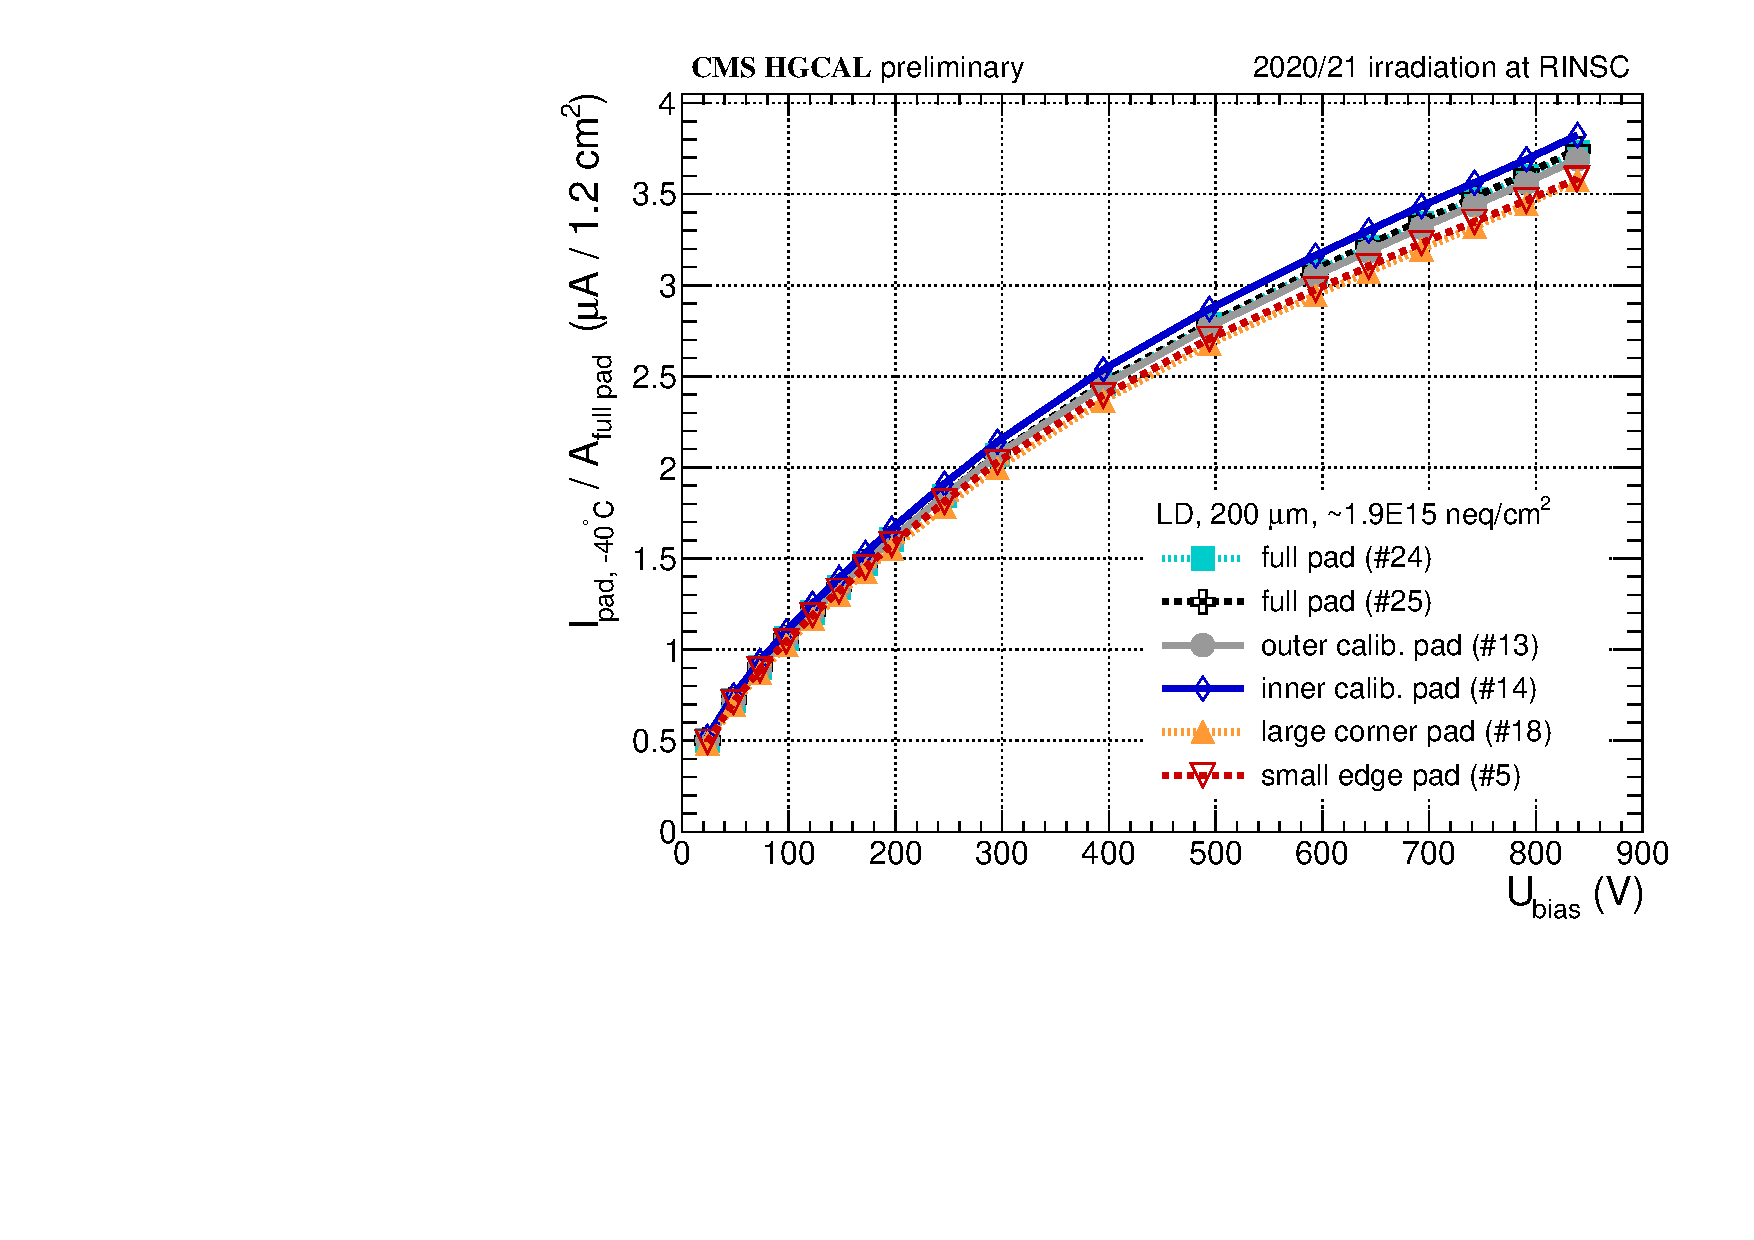
\includegraphics[width=0.999\textwidth]{plots/channel_iv/channel_IV_sensors_channels.pdf}
        \subcaption{
        }
        \label{plot:pad_IV_channels}
    \end{subfigure}

	\caption{
		(a) Total leakage currents after irradiation (without additional annealing) for two representative example sensors. 
		Currents were measured at \SI{-40}{\celsius} ($\text{I}_\text{tot, \SI{-40}{\celsius}}$) and at different effective bias voltages ($\text{U}_\text{bias}$). 
        (b) Per-pad leakage currents normalised to the area of full hexagonal pads as a function of the effective bias voltage for different pads with different geometries on one example sensor.
	}
\end{figure}
The total leakage current is defined as the current flowing through the high-voltage resistor R$_\text{HV}$ (cf. Figure 2 in~\cite{pitters:array2019}) and is interpreted as the dark current of a full silicon sensor.
As it is exemplified for two prototype sensors in \ref{plot:tot_IV_good}, the total leakage current did not exhibit exponential growth and stayed well below the ARRAY system's compliance of \SI{2}{\milli\ampere} for most of the irradiated sensors that were tested up to \SI{850}{\volt} at \SI{-40}{\celsius}.
Irreversible discharges are undesired but in fact occurred for a handful of the tested sensors where the total leakage current during electrical characterisation suddenly increased and exceeded the \SI{2}{\milli\ampere} limitation.
Whereas one half of those instances could be traced back mechanical damages, e.g.$~$induced during the transport (from RINSC to CERN), the other half hinted at the presence of a minor flaw in the HGCAL silicon sensor design.
The latter ultimately lead to a design modification with which the risk of discharges in the future should be minimised\footnote{More than 50 prototype sensors with the improved design have been characterized with voltages up to \SI{850}{\volt} in the meantime. None have shown discharges thus far.}.
Results of the affected sensors are not discussed further in this work.
\ref{plot:pad_IV_channels} shows the per-pad leakage current as a function of the effective bias voltage (\emph{IV}) for adjacent pads on one representative low density sensor irradiated to intermediate fluences.
The data demonstrate that the leakage current of a pad after irradiation scales with its volume, and that the relative increase from \SI{600}{\volt} to \SI{800}{\volt} remains well below \SI{150}{\percent}.
The beneficial effect of annealing on the leakage current has been studied in more detail for a sensor which was not exposed to high temperatures during irradiation.
The measured IV curves after different annealing times are shown for a representative pad in \ref{plot:annealing_IV}.
\begin{figure}
	\captionsetup[subfigure]{aboveskip=-1pt,belowskip=-1pt}
	\centering
	\begin{subfigure}[b]{0.49\textwidth}
		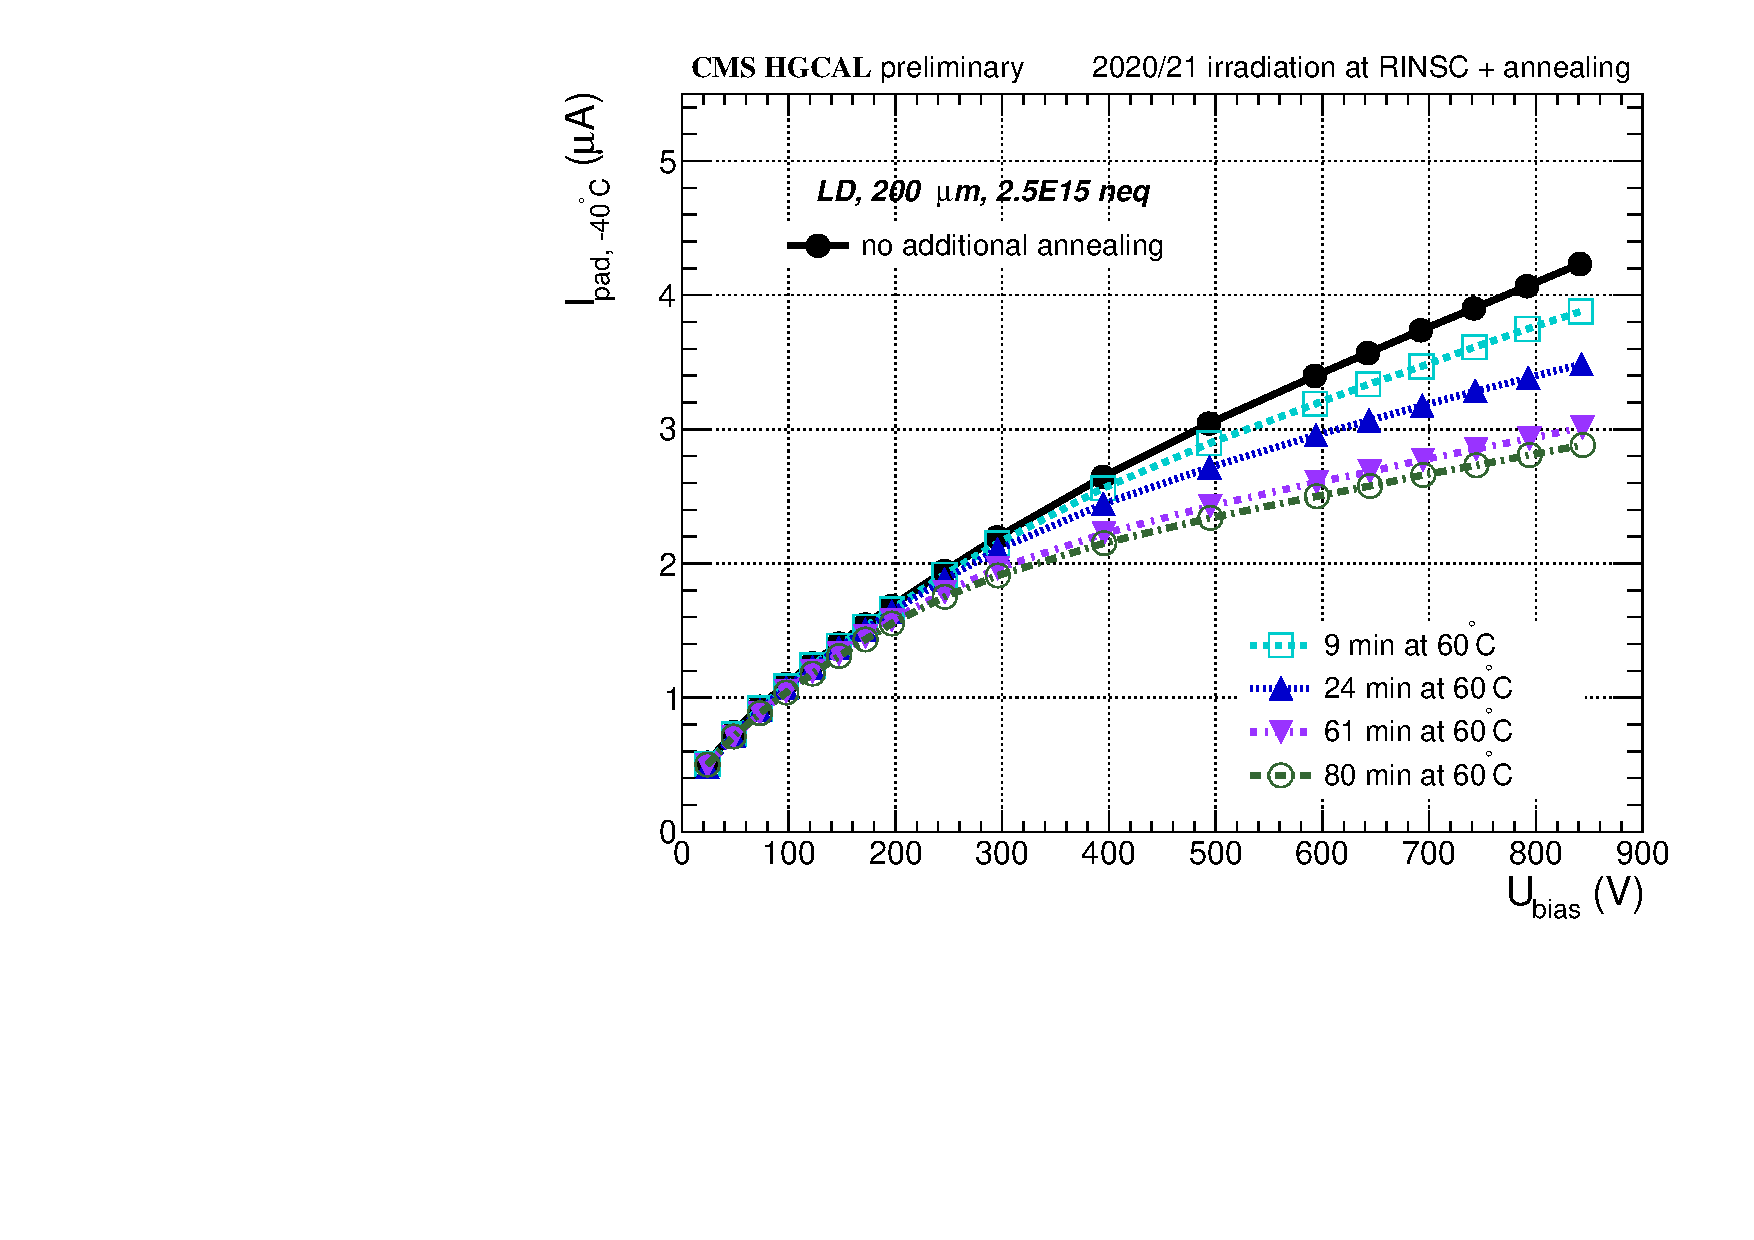
\includegraphics[width=0.999\textwidth]{plots/annealing_iv/annealing_IV_ch24.pdf}
		\subcaption{
		}
		\label{plot:annealing_IV}
	\end{subfigure}
	\hfill
	\begin{subfigure}[b]{0.49\textwidth}
		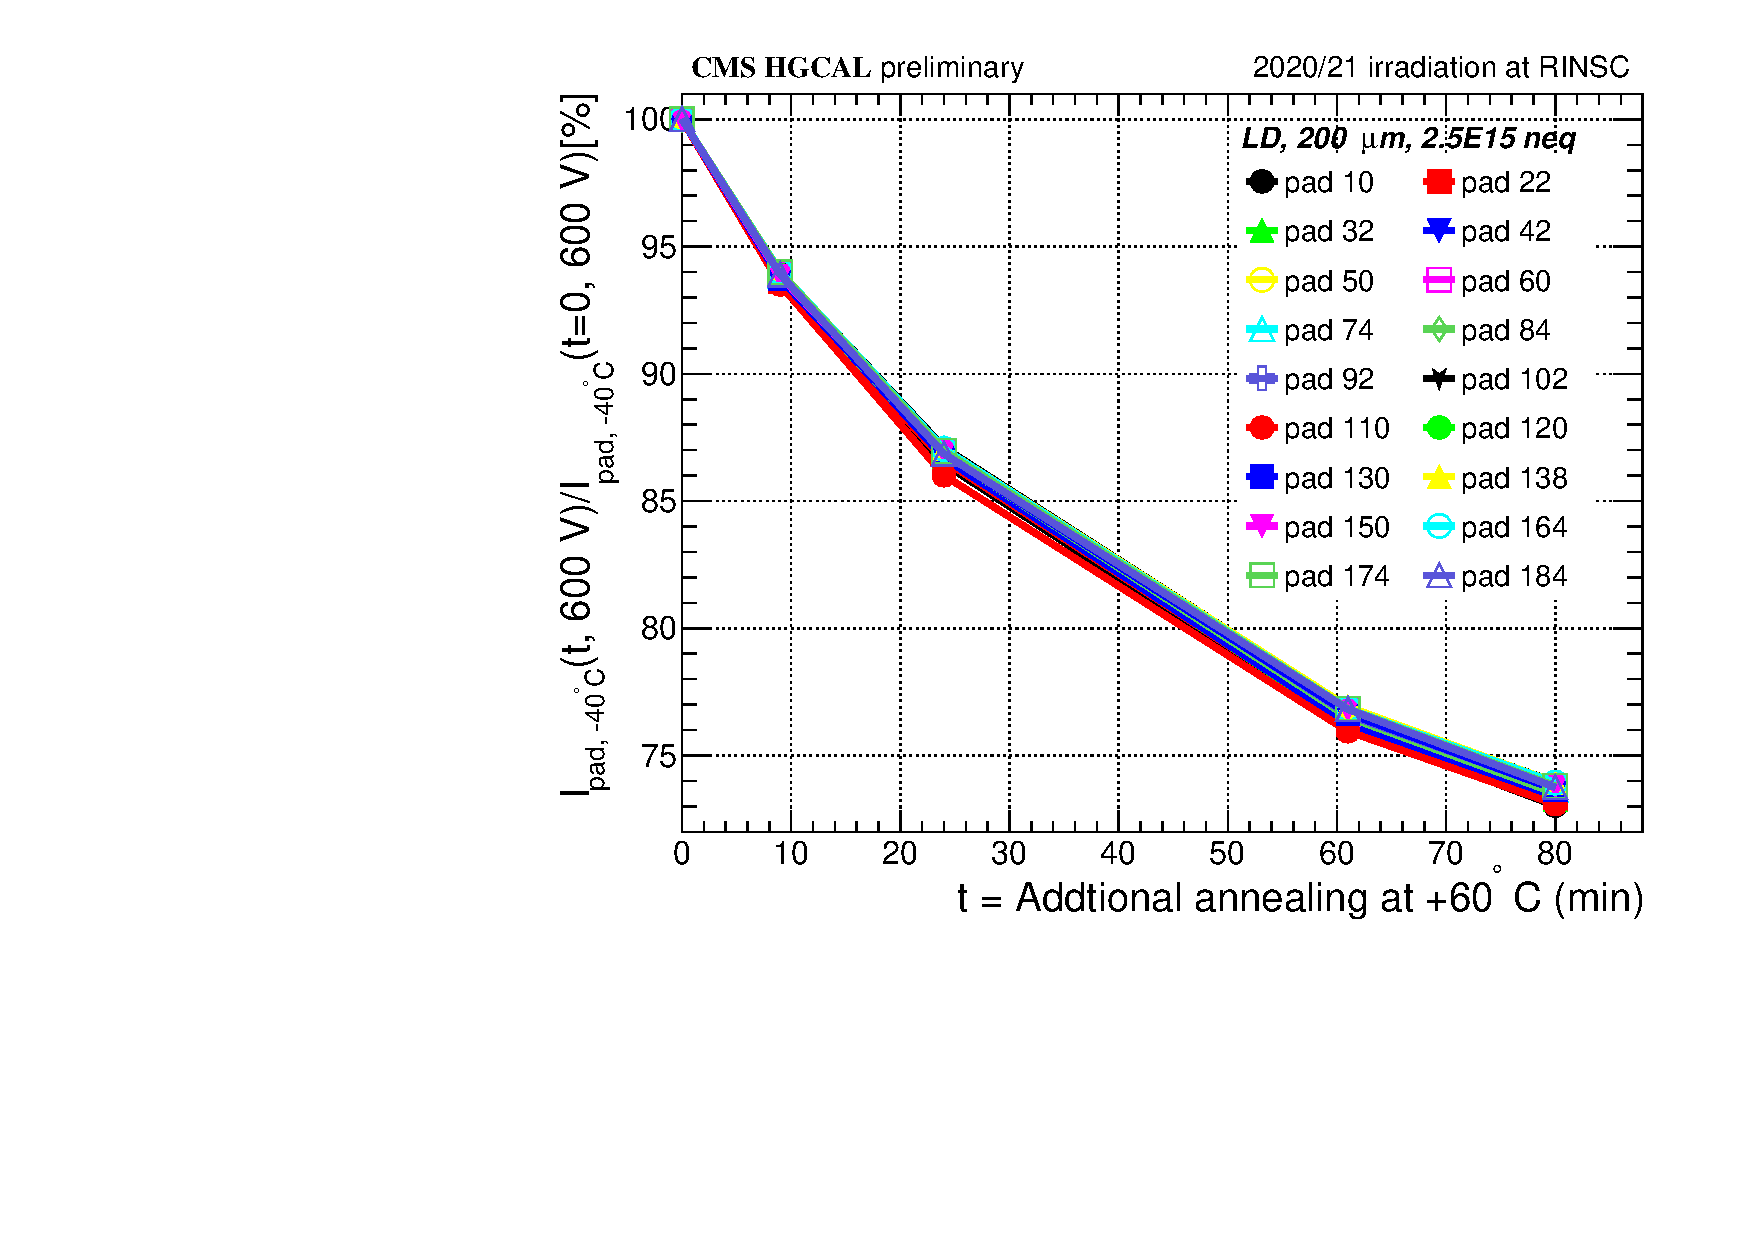
\includegraphics[width=0.999\textwidth]{plots/annealing_iv/annealing_current.pdf}
		\subcaption{
		}
		\label{plot:annealing_current}
	\end{subfigure}    

	\caption{
		(a) IV-curves of a representative full hexagonal pad for different annealing scenarios for a \SI{200}{\micro\metre} low-density prototype sensor irradiated to approximately 2.4$~$E15~$\neqcm$.
        (b) Decrease of the per-pad leakage current (interpolated to $U_\text{bias}=\SI{600}{\volt}$) as a function of the annealing time at \SI{60}{\celsius} for a subset of full hexagonal pads that are uniformly distributed over the full sensor.
	}
\end{figure}
For bias voltages beyond full depletion, per-pad leakage currents at \SI{600}{\volt} are reduced systematically by \SI{25}{\percent} after \SI{80}{\minute} at \SI{60}{\celsius}, cf.~\ref{plot:annealing_current}.
Given the simultaneous reduction in the depletion voltage, cf.~\ref{plot:annealing_CV}, leakage currents around full depletion are even reduced further.
Altogether, we observe the expected proportionality of the per-pad leakage current density to the anticipated fluence that the sensors were exposed to.
The proportionality for current densities interpolated to an effective bias voltage of \SI{600}{\volt}, which is well above full depletion for most of the investigated sensors, and extrapolated to HGCAL's foreseen operation temperature of \SI{-30}{\celsius} is displayed in \ref{plot:alpha_600}.
\begin{figure}
	\captionsetup[subfigure]{aboveskip=-1pt,belowskip=-1pt}
	\centering
    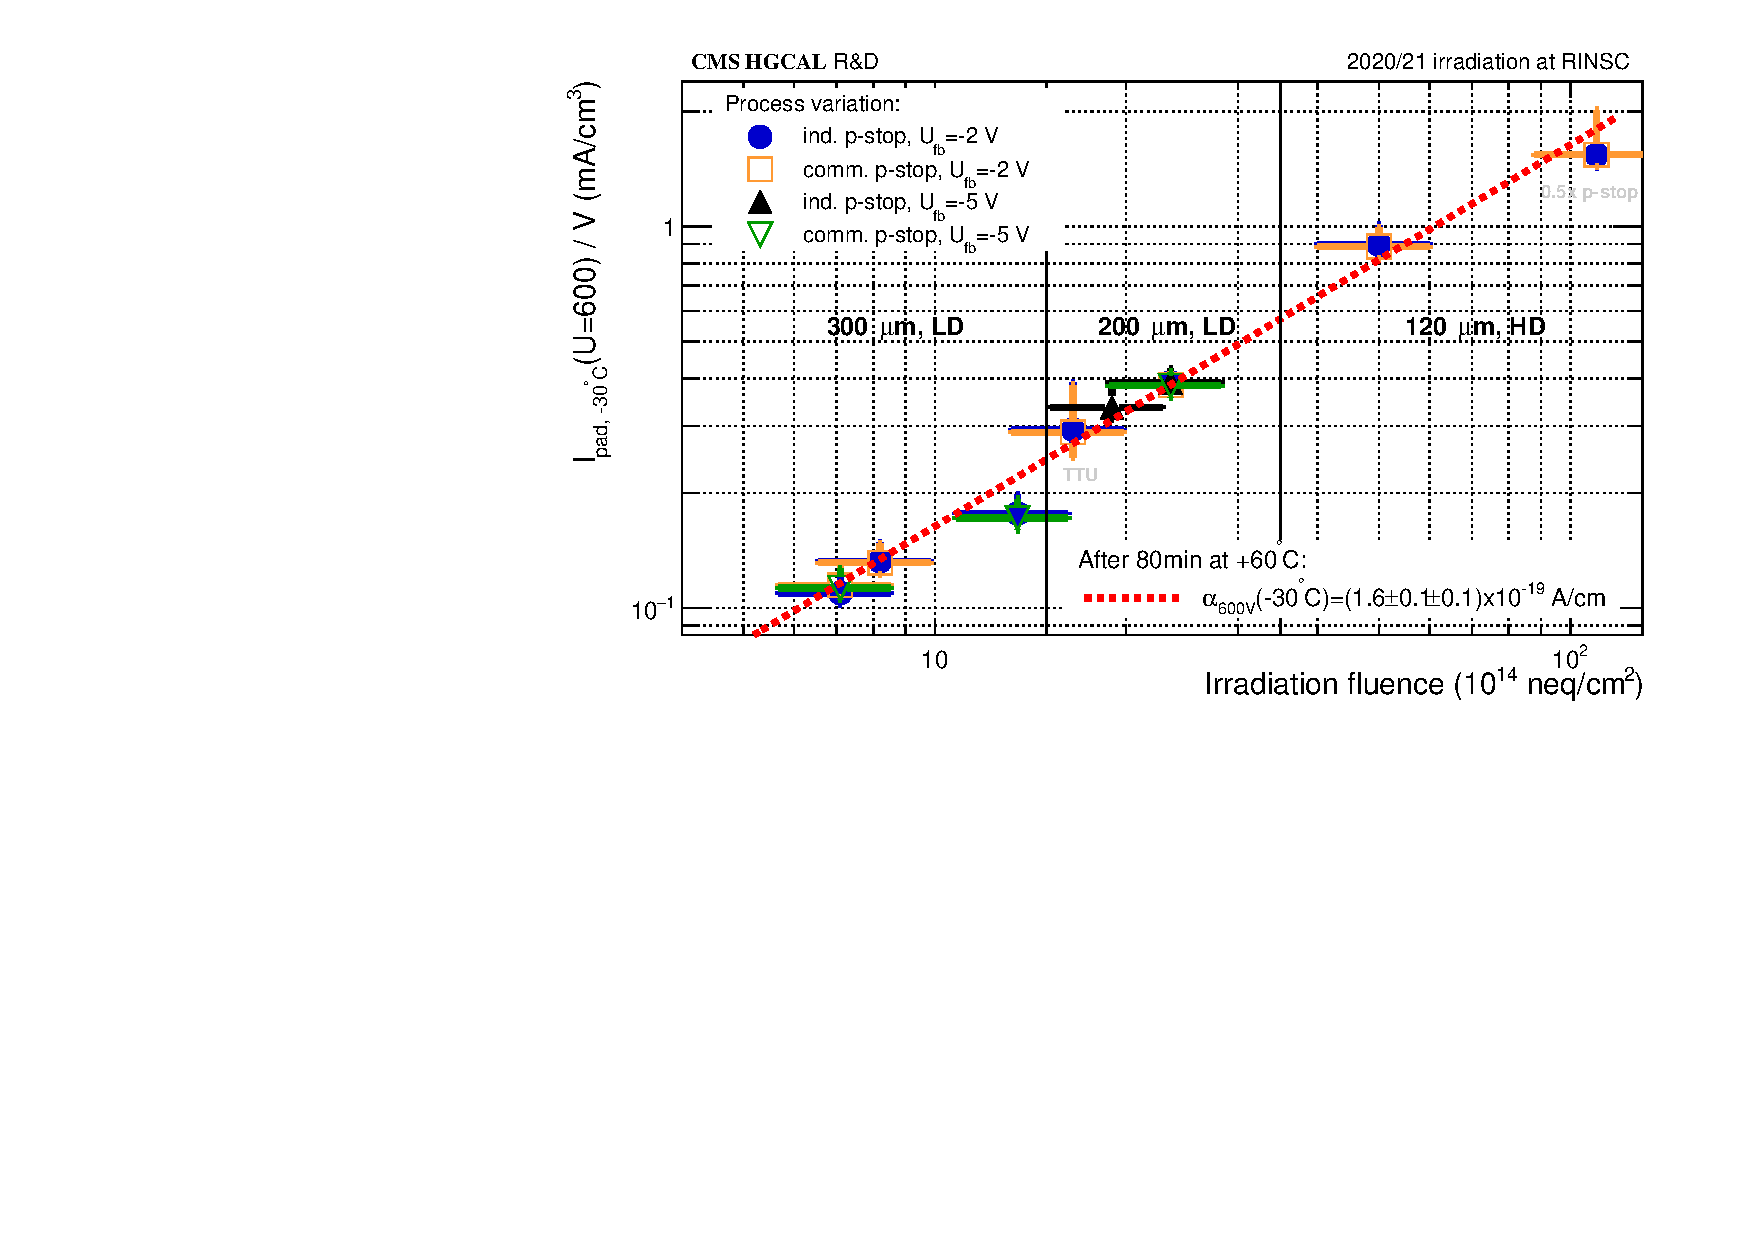
\includegraphics[width=0.69\textwidth]{plots/alpha/alpha_600V.pdf}
	\caption{
		Volume-normalised per-pad leakage currents interpolated to an effective bias voltage of \SI{600}{\volt} as a function of the fluence that they were exposed to.
        The quoted currents were measured after additional annealing at \SI{60}{\celsius}, and are scaled to HGCAL's foreseen operation temperature of \SI{-30}{\celsius}.
		"TTU" denotes the measurements of a \SI{120}{\micro\meter} HD sensor conducted with a setup, analogous to the one described in~\ref{subsec:setup_alps}, at Texas Tech University. 
		Those exhibit overall consistency with the measurements conducted with the setup at CERN.
		}
	\label{plot:alpha_600}
\end{figure}
As expected~\cite{MOLL199987}, the current-related damage rate ($\alpha$) is found to be independent of the silicon material properties investigated in this work.
%However, the numerical result for $\alpha$ is about \SI{15}{\percent} smaller than the literature value~\cite{moll:SiDamages}, hereby potentially indicating a systematic overestimate of the fluence at the RINSC irradiation facility. 
Interestingly, even after correction for the chuck temperature non-uniformity, per-pad leakage current densities across a sensor at a fixed voltage differ by up to \SI{20}{\percent}.
The associated current profiles are present both before (cf. \ref{plot:iv_hexplot_3009,plot:iv_hexplot_0541_04,plot:iv_hexplot_1013}) and after additional annealing (cf. \ref{plot:iv_hexplot_3009_annealed,plot:iv_hexplot_0541_04_annealed,plot:iv_hexplot_1013_annealed}).
Furthermore, they are consistent between sensors that had been irradiated simultaneously in the same puck.
Hence, this circumstance is interpreted as evidence for the presence of a gaussian-like ($\sigma\approx\SI{10}{\centi\metre}$) fluence profile within the beam port of the irradiation facility at RINSC.
\begin{figure}
	\captionsetup[subfigure]{aboveskip=-1pt,belowskip=-1pt}
	\centering
	\begin{subfigure}[b]{0.32\textwidth}
		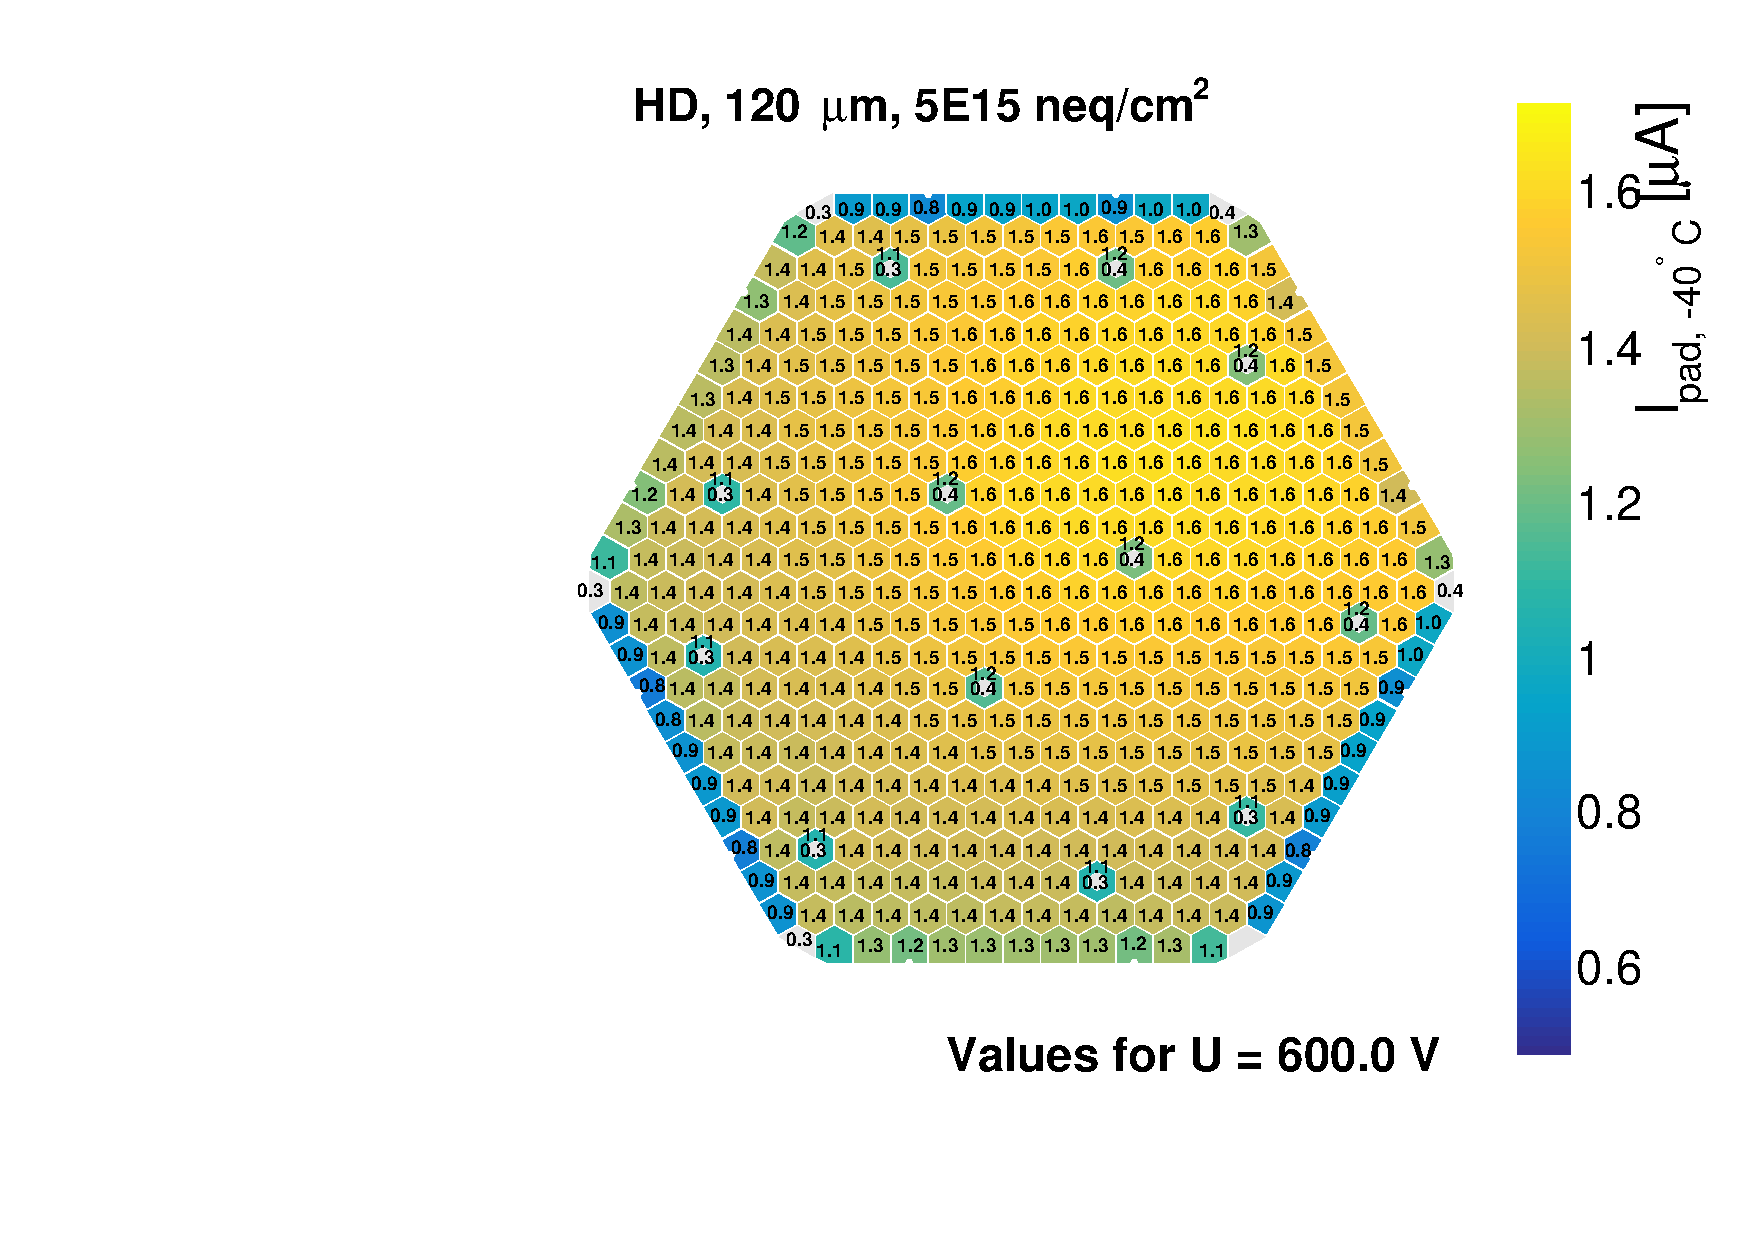
\includegraphics[width=0.999\textwidth]{plots/iv_hexplots/3009.pdf}
		\subcaption{
		}
		\label{plot:iv_hexplot_3009}
	\end{subfigure}
	\hfill
	\begin{subfigure}[b]{0.32\textwidth}
		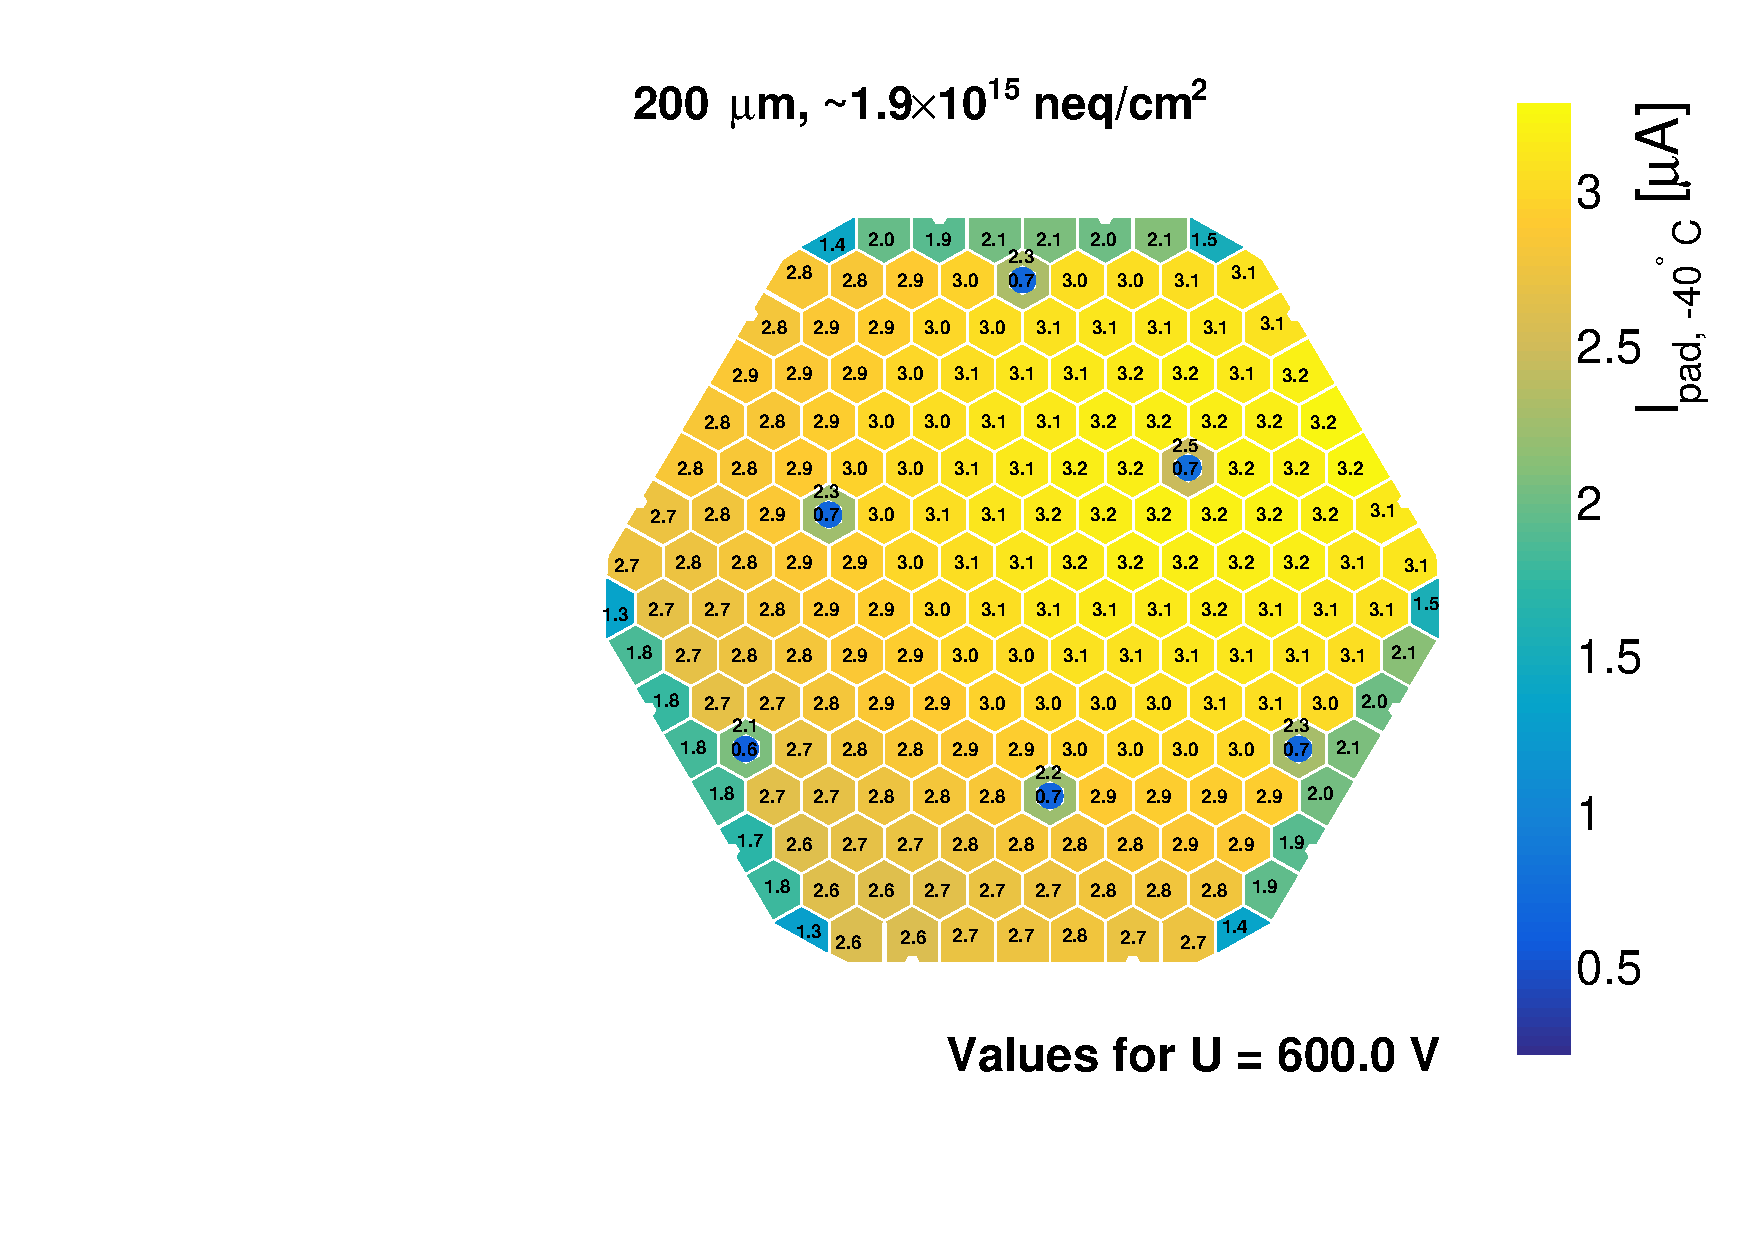
\includegraphics[width=0.999\textwidth]{plots/iv_hexplots/0541_04.pdf}
		\subcaption{
		}
		\label{plot:iv_hexplot_0541_04}
	\end{subfigure}
	\hfill	
	\begin{subfigure}[b]{0.32\textwidth}
		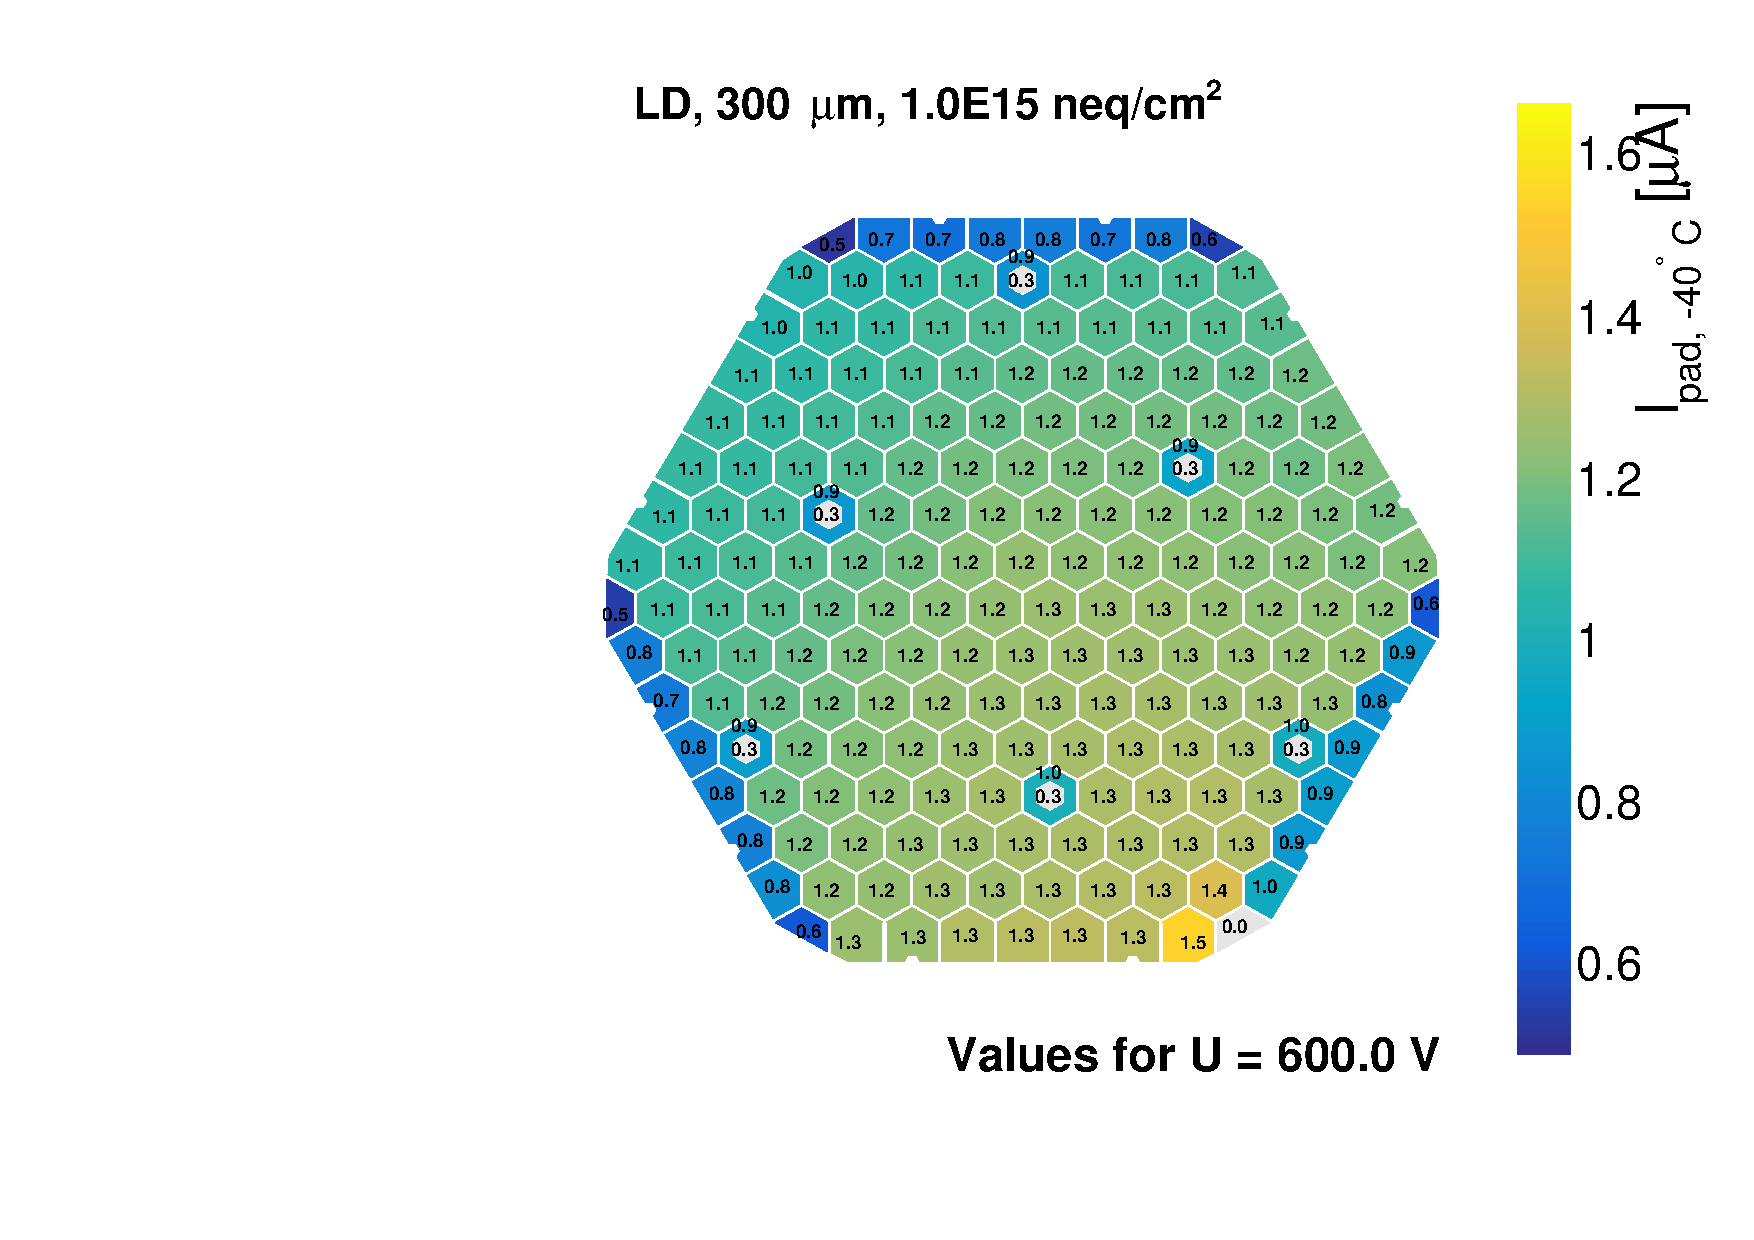
\includegraphics[width=0.999\textwidth]{plots/iv_hexplots/1013.pdf}
		\subcaption{
		}
		\label{plot:iv_hexplot_1013}
	\end{subfigure}
    \hfill
	\begin{subfigure}[b]{0.32\textwidth}
		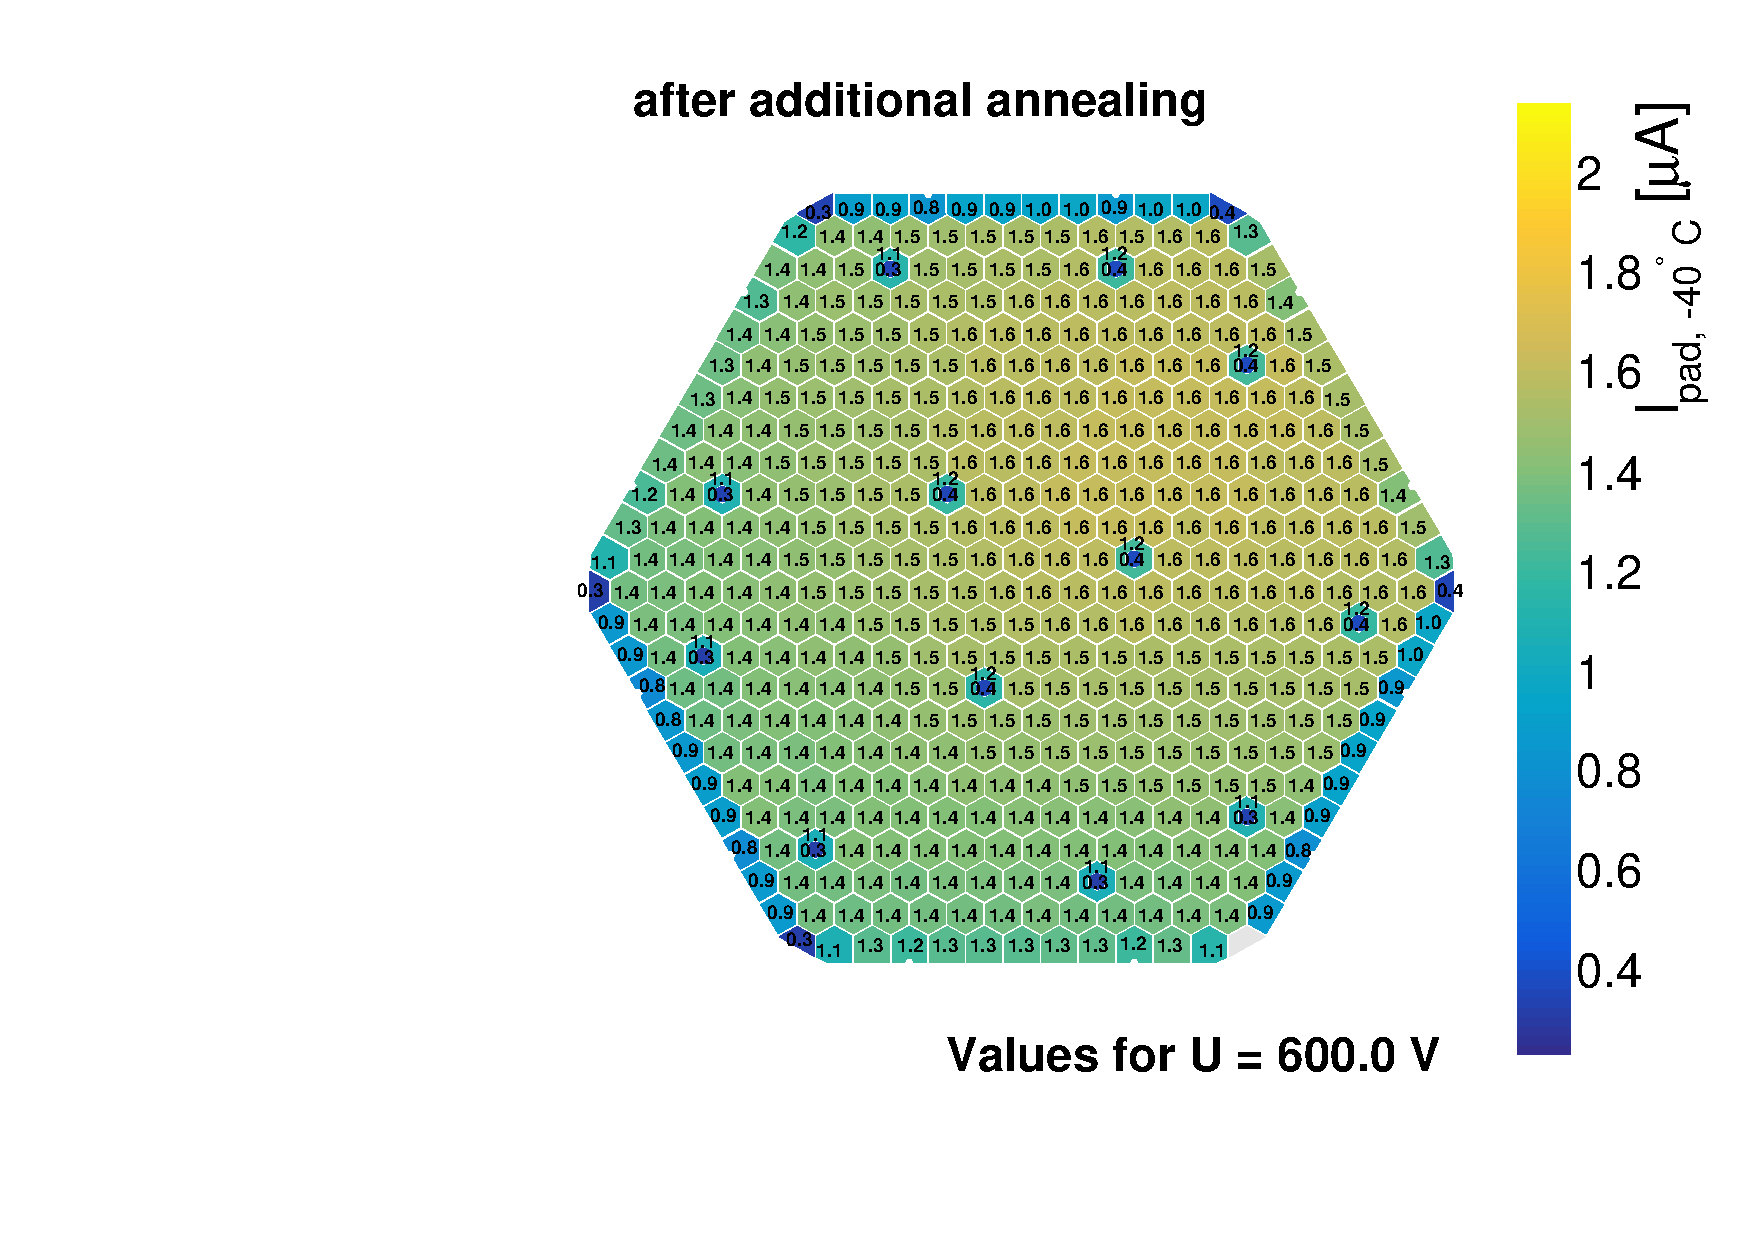
\includegraphics[width=0.999\textwidth]{plots/iv_hexplots/3009_annealed.pdf}
		\subcaption{
		}
		\label{plot:iv_hexplot_3009_annealed}
	\end{subfigure}
	\hfill
	\begin{subfigure}[b]{0.32\textwidth}
		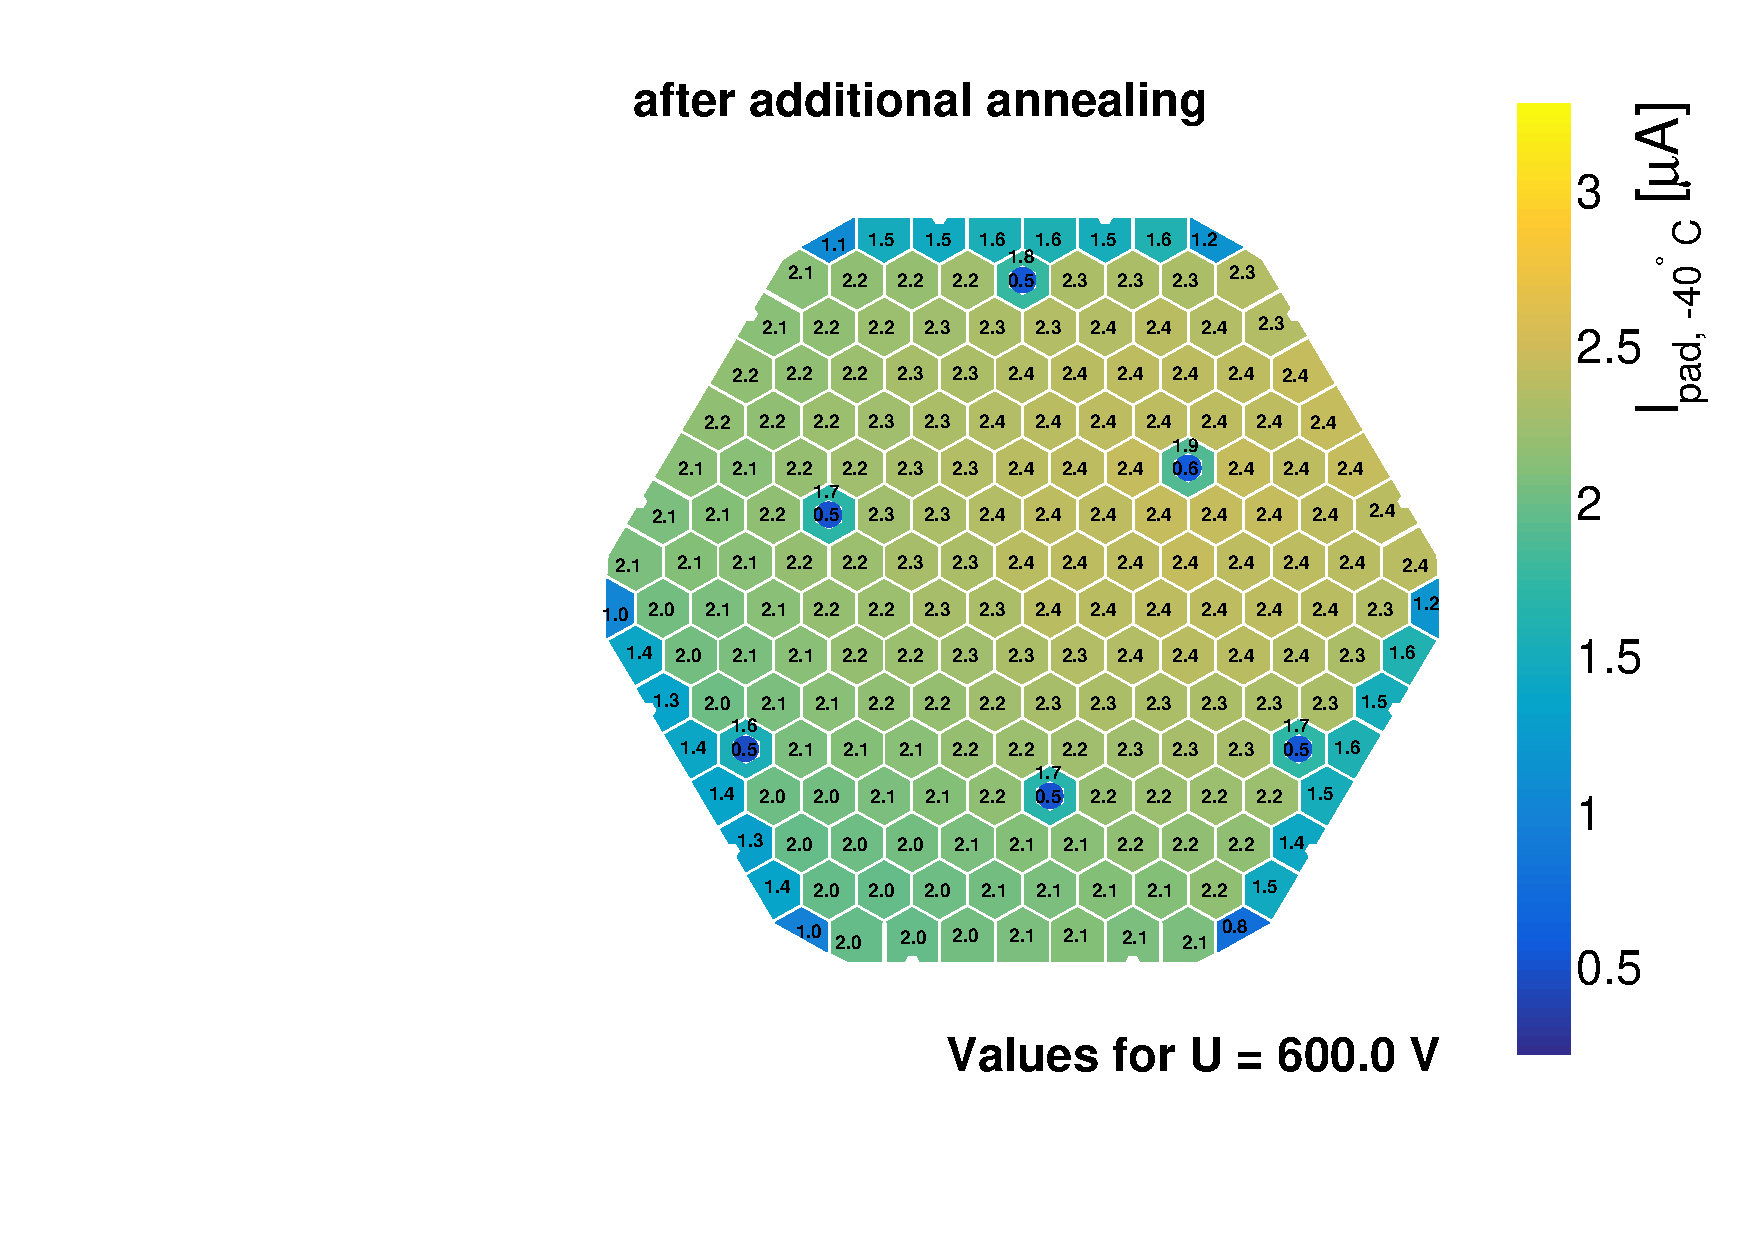
\includegraphics[width=0.999\textwidth]{plots/iv_hexplots/0541_04_annealed.pdf}
		\subcaption{
		}
		\label{plot:iv_hexplot_0541_04_annealed}
	\end{subfigure}
	\hfill	
	\begin{subfigure}[b]{0.32\textwidth}
		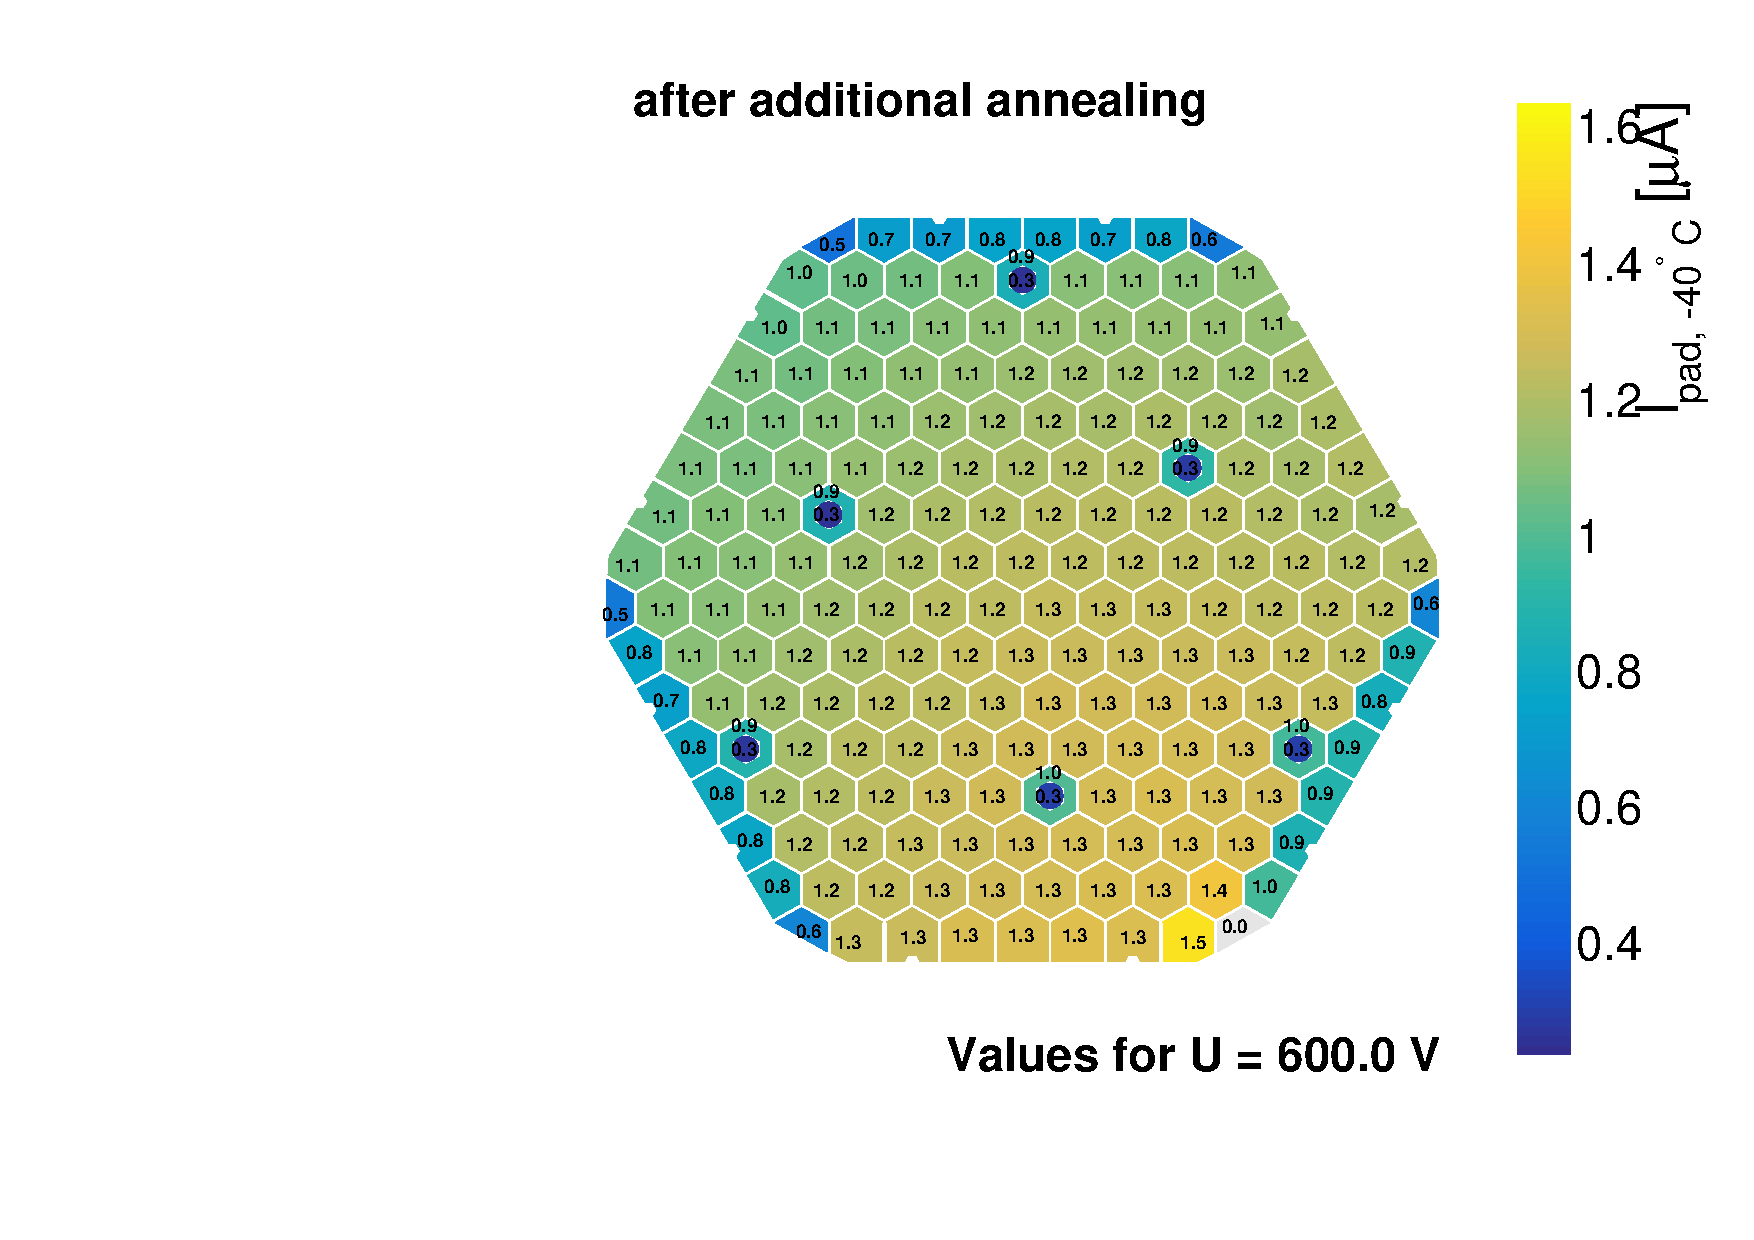
\includegraphics[width=0.999\textwidth]{plots/iv_hexplots/1013_annealed.pdf}
		\subcaption{
		}
		\label{plot:iv_hexplot_1013_annealed}
	\end{subfigure}    
	\caption{
		Per-pad leakage currents interpolated to an effective bias voltage of \SI{600}{\volt} for three representative sensors from different irradiation rounds before (a-c) and after additional annealing (d-f).
		Red- or white-colored edge pads correspond to well-understood measurement effects, e.g. insufficient contact between the pogo pins and the pads.
		}
	\label{plot:iv_hexplot}
\end{figure}


\subsection{Capacitance and Depletion Voltage}
\label{subsec:Udep}
The measured per-channel impedance is open-corrected by subtracting the impedance of the ARRAY system.
Subsequently, the sensor pad capacitance is computed assuming an underlying serial circuitry.
Due to the finite mobility of the sensor defects, the frequency at which the impedance is measured may, in principle, have sizeable impact on the hereby derived capacitance and on the depletion voltages for irradiated silicon pad sensors, cf. Ref.~\cite{Li1991}.
The impedance measurement for the results presented in this section was conducted at an LCR-frequency ($f_\text{LCR}$) of \SI{2}{\kilo\hertz}.
Experimental follow-up studies indicate a negligible impact of \SI{2}{\percent} on the asymptotic capacitance and a \SI{10}{\percent} reduction of the depletion voltage when decreasing $f_\text{LCR}$ to \SI{500}{\hertz}.
This dependence on $f_\text{LCR}$ has no practical implications on the following discussion.
The depletion voltage for each pad is assessed from the saturation of its squared reciprocal capacitance ($C^{-2}$) of a pad with respect to the effective bias voltage ($V$). 
It is defined as the intersection of a straight-line fitted to the rising part of the $C^{-2}$ vs. $V$ curve with a line fitted to its plateau.
Prior to additional annealing, such a plateau could not always be reached within the tested bias voltage range, see for example the black line in \ref{plot:annealing_CV}. 
After additional annealing to \SI{80}{\min} at \SI{60}{\celsius}, the estimated depletion voltage has been reduced by about a third with respect to the case without annealing, cf.~\ref{plot:annealing_Vdep}.
Only results from sensors after additional annealing are discussed in the following. 
\begin{figure}
	\captionsetup[subfigure]{aboveskip=-1pt,belowskip=-1pt}
	\centering

	\begin{subfigure}[b]{0.49\textwidth}
		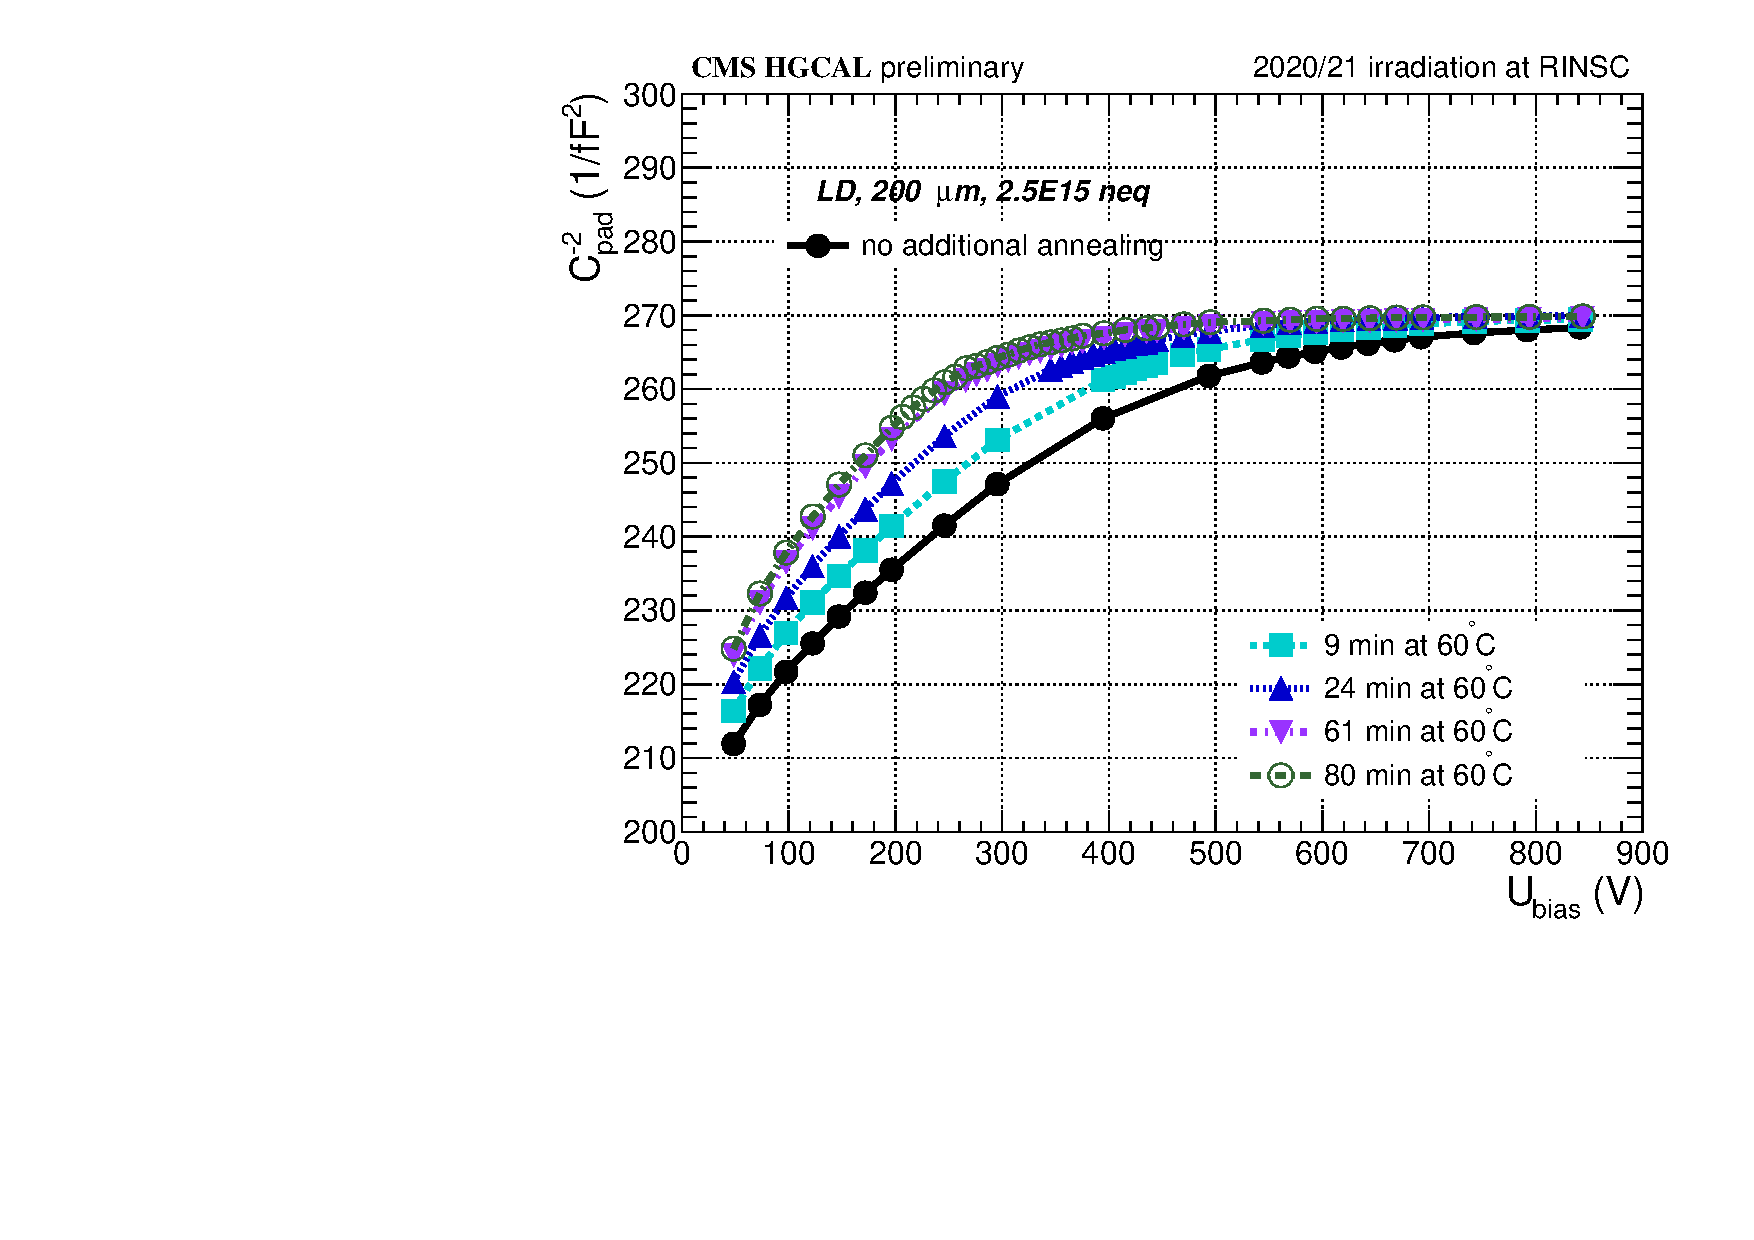
\includegraphics[width=0.999\textwidth]{plots/annealing_Vdep/annealing_CV_ch24.pdf}
		\subcaption{
		}
        \label{plot:annealing_CV}
	\end{subfigure}
    \hfill
    \begin{subfigure}[b]{0.49\textwidth}
		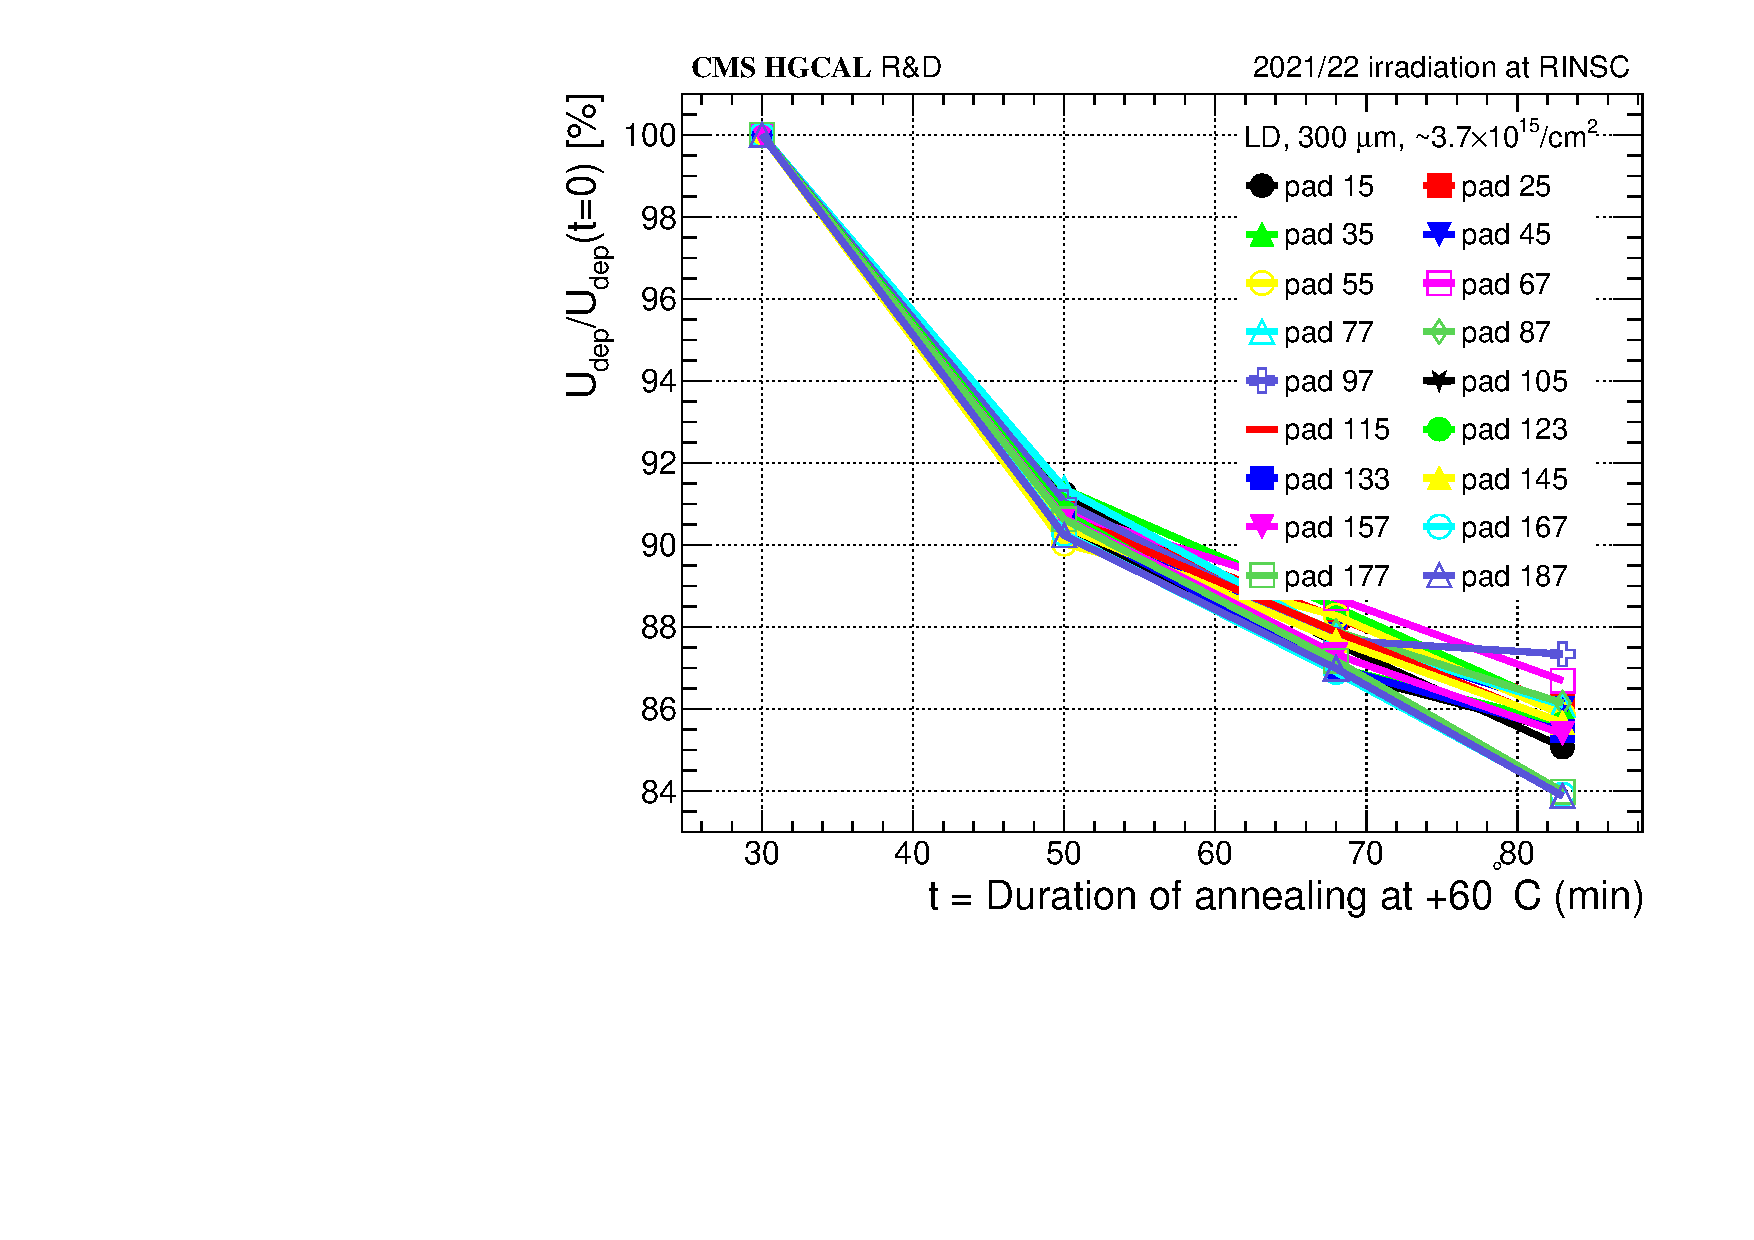
\includegraphics[width=0.999\textwidth]{plots/annealing_Vdep/annealing_Vdep.pdf}
		\subcaption{
		}		
        \label{plot:annealing_Vdep}
	\end{subfigure}
	\caption{
        (a) Reciprocal-squared capacitance ($C^2_\text{pad}$) as a function the bias voltage of a representative full hexagonal pad for different annealing scenarios for a \SI{200}{\micro\metre} low-density prototype sensor irradiated to approximately 2.4$~$E15~$\neqcm$.   
		(b) Relative decrease of the depletion voltage estimate ($U_\text{dep}$) as a function of the additional annealing time at \SI{60}{\celsius} for a subset of full pads.
	}
\end{figure}
\begin{figure}
	\captionsetup[subfigure]{aboveskip=-1pt,belowskip=-1pt}
	\centering
	\begin{subfigure}[b]{0.49\textwidth}
		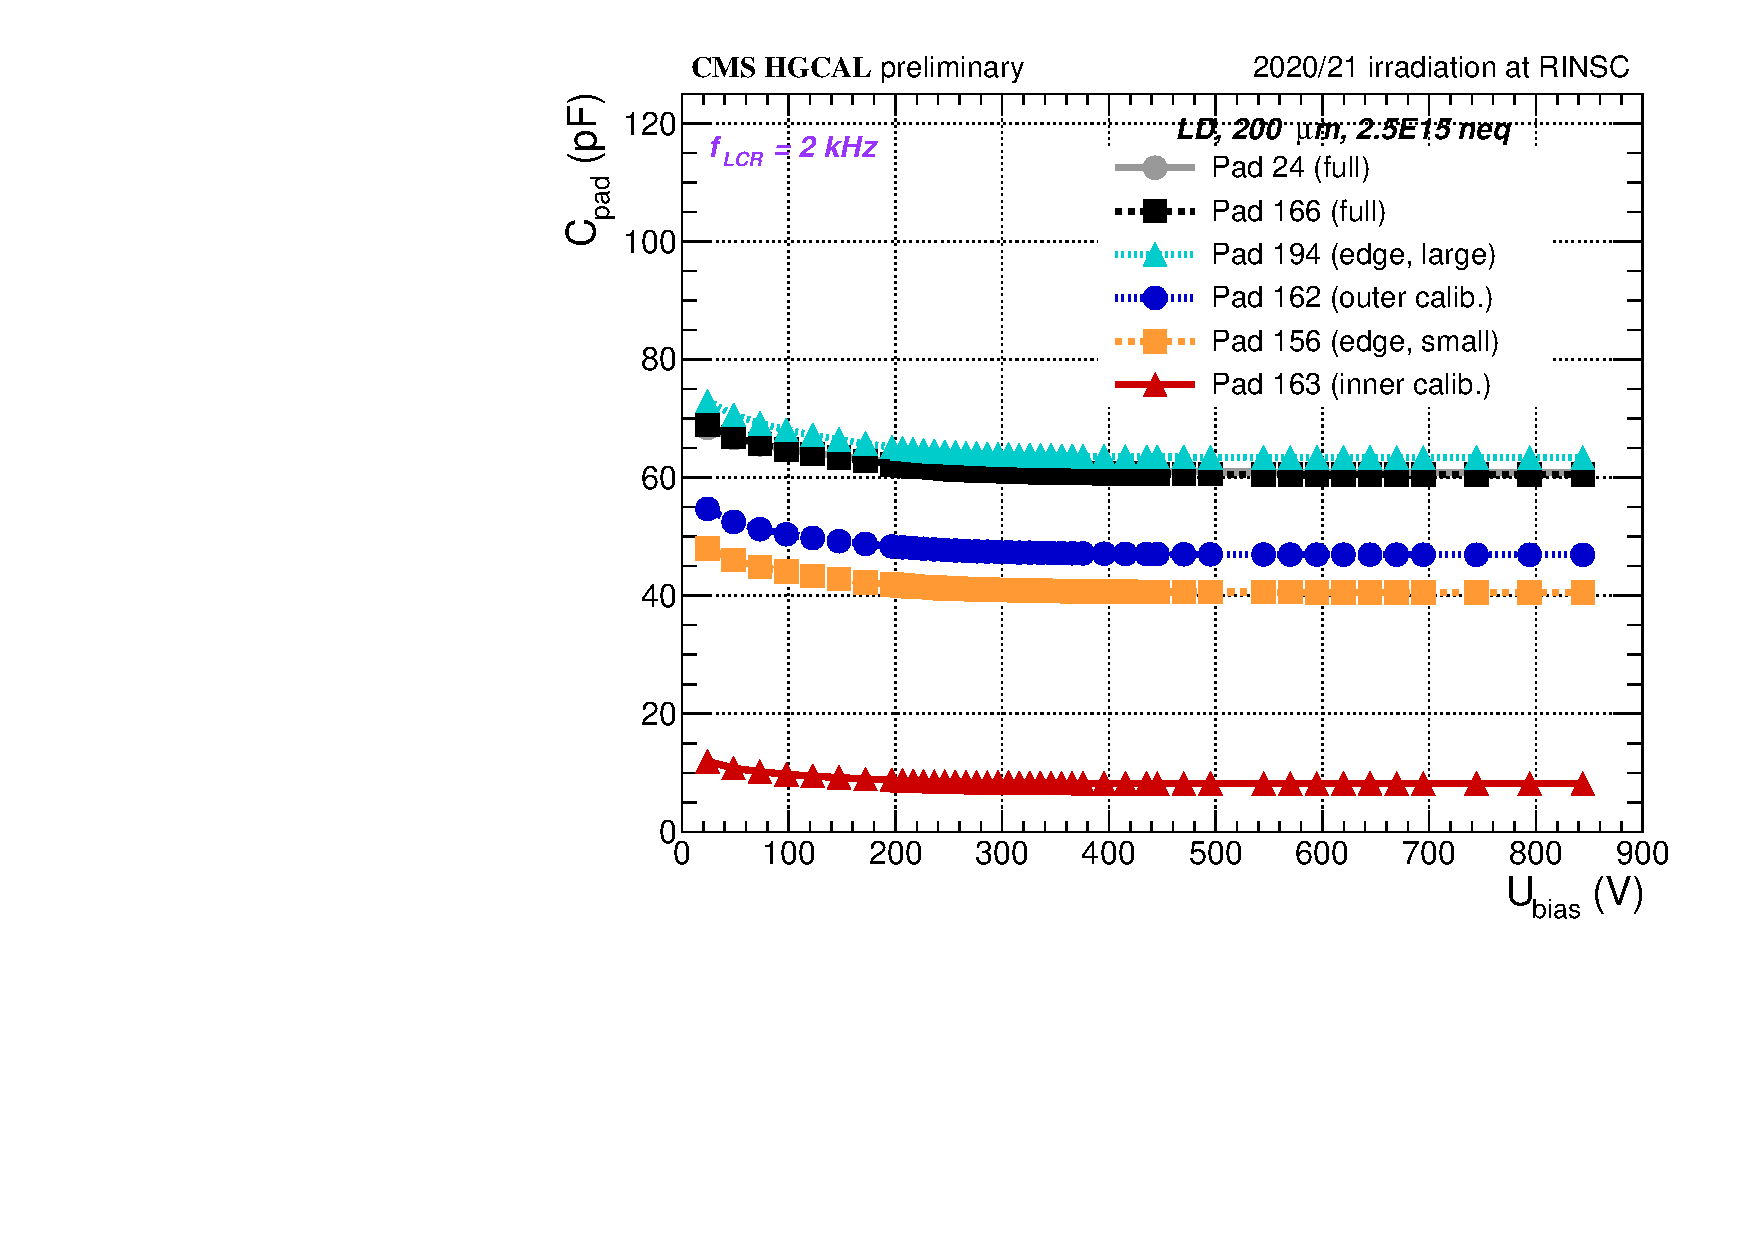
\includegraphics[width=0.999\textwidth]{plots/channel_cv/channel_CV_sensors_channels.pdf}
		\subcaption{
		}
		\label{plot:pad_CV_channels}
	\end{subfigure}
	\hfill
	\begin{subfigure}[b]{0.49\textwidth}
		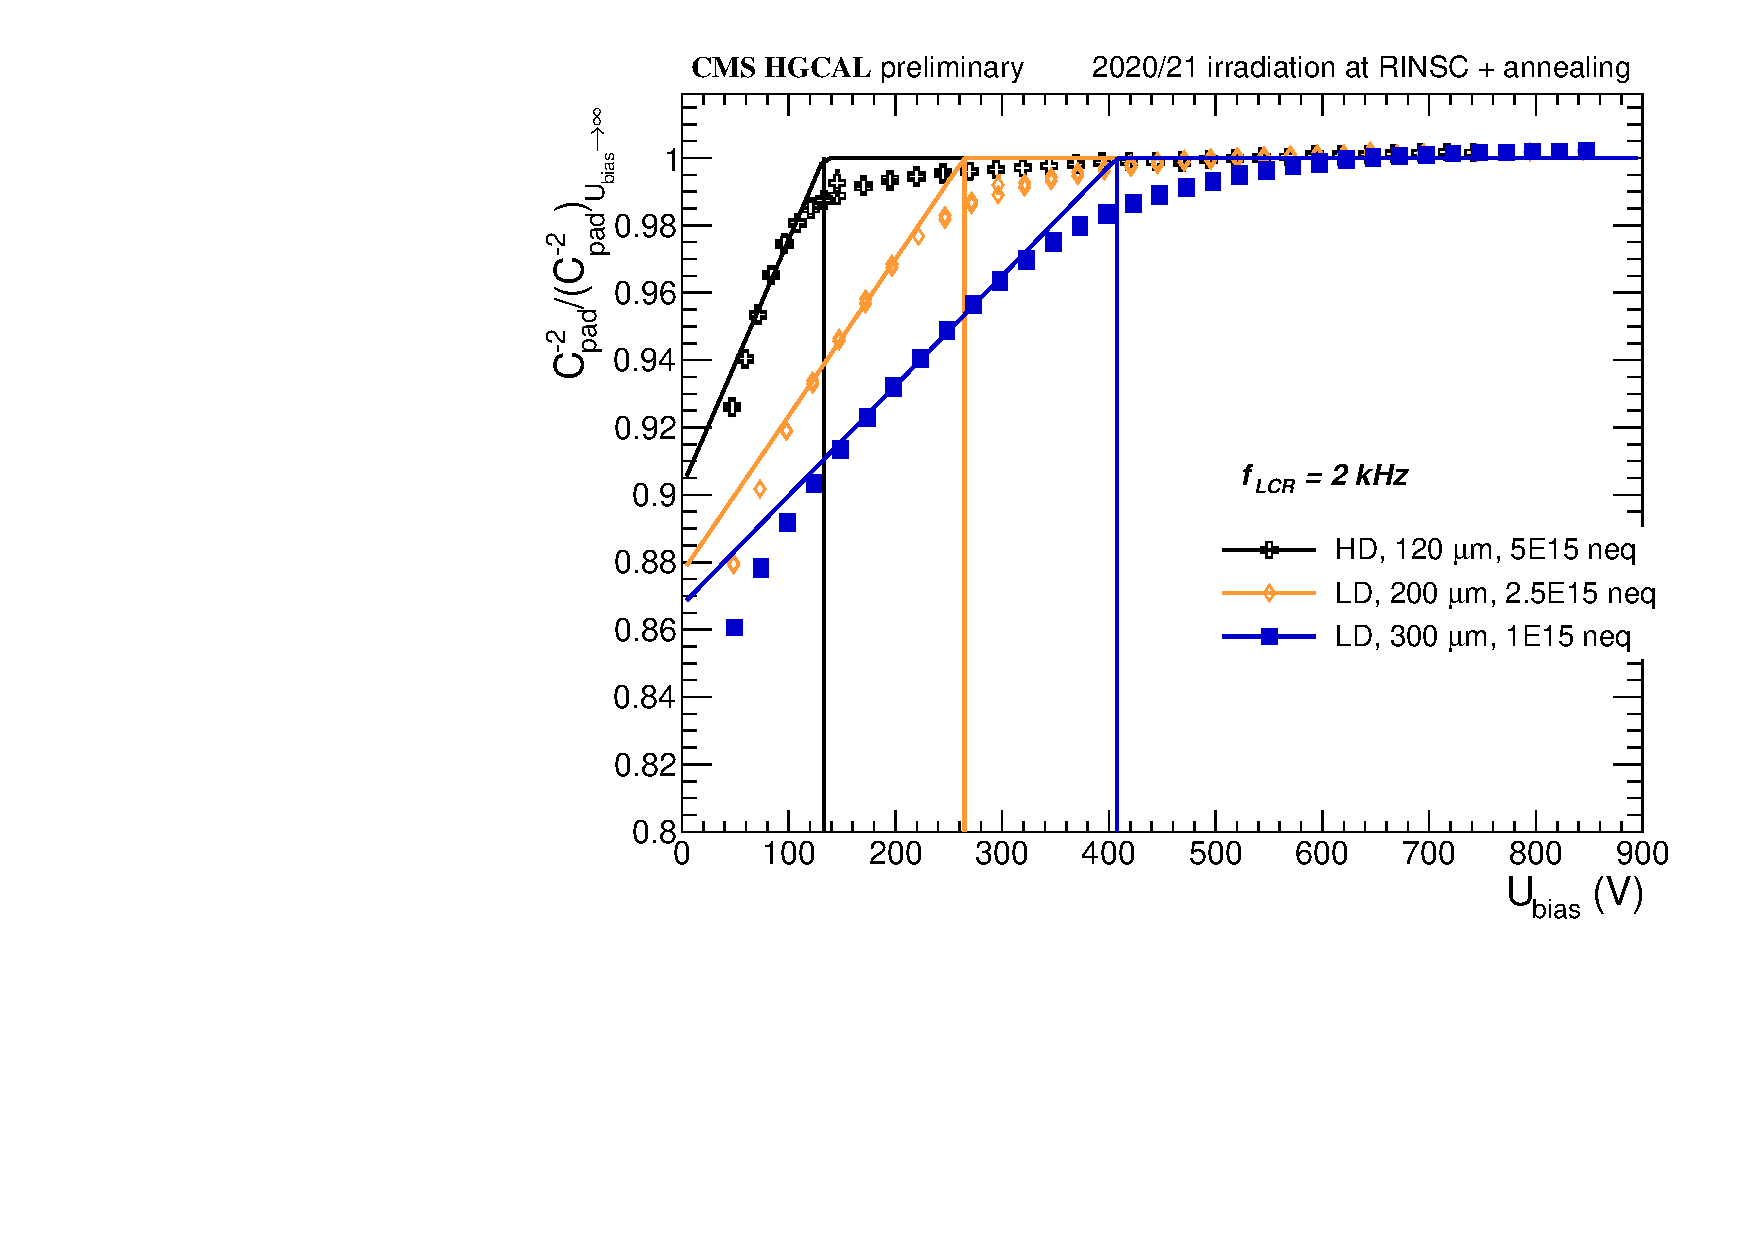
\includegraphics[width=0.999\textwidth]{plots/channel_cv/channel_invCV_sensors_sensors.pdf}
		\subcaption{
		}
		\label{plot:pad_invCV_sensor}
	\end{subfigure}
	\caption{
		(a) Area-normalised capacitances as a function of the effective bias voltage for different pads with different geometries on one example low density sensor.
		(b) Normalised squared-inverse capacitances as a function of the effective bias voltage for estimating the sensor depletion voltage for one central pad on three example sensors from different irradiation rounds.
		The frequency of the Keysight E4980A LCR meter in these measurements was set to \SI{2}{\kilo\hertz}.
	}
\end{figure}
\begin{figure}
	\captionsetup[subfigure]{aboveskip=-1pt,belowskip=-1pt}
	\centering
	\begin{subfigure}[b]{0.49\textwidth}
		\centering
		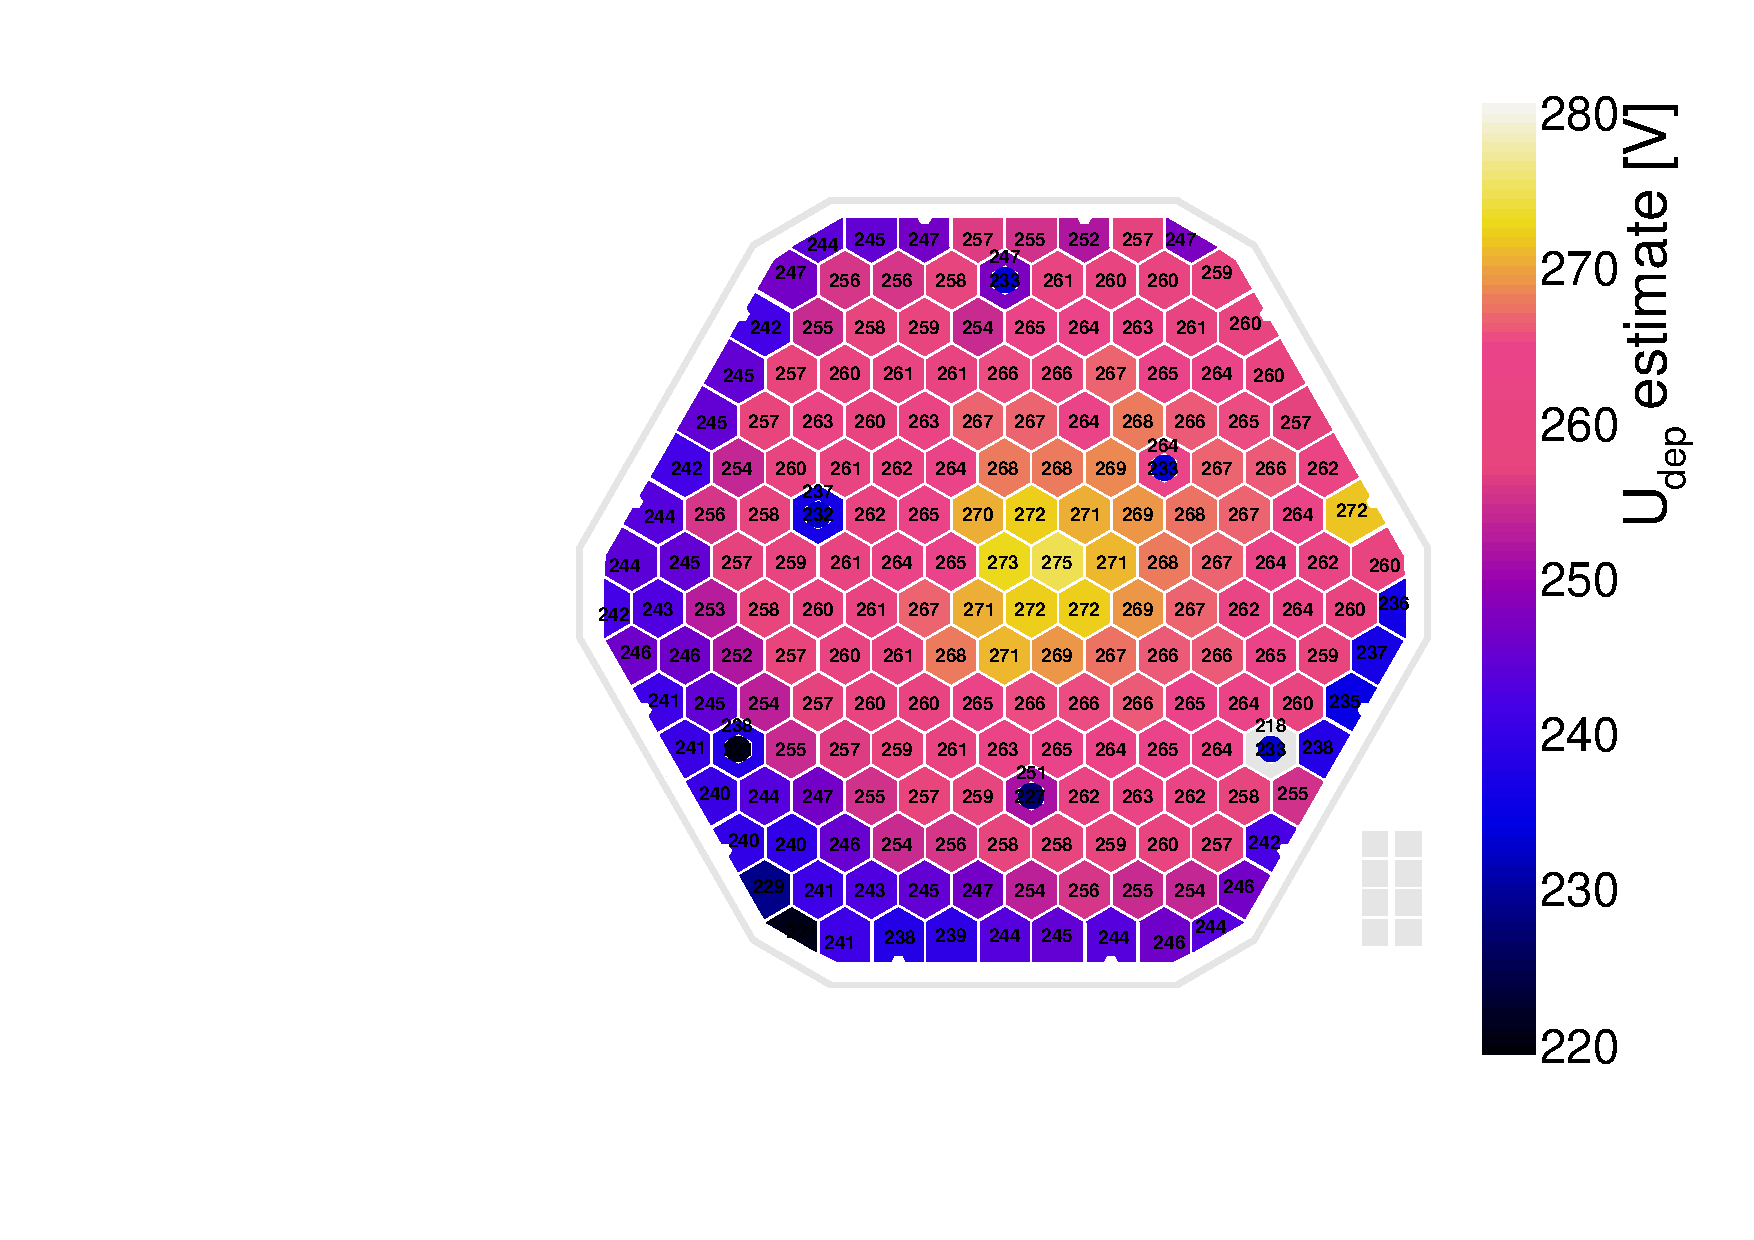
\includegraphics[width=0.99\textwidth]{plots/Vdep_hexplots/0541_04.pdf}
		\subcaption{
			}
			\label{plot:Vdep_hexplot_0541_04}
	\end{subfigure}
	\hfill
	\begin{subfigure}[b]{0.49\textwidth}
		\centering
		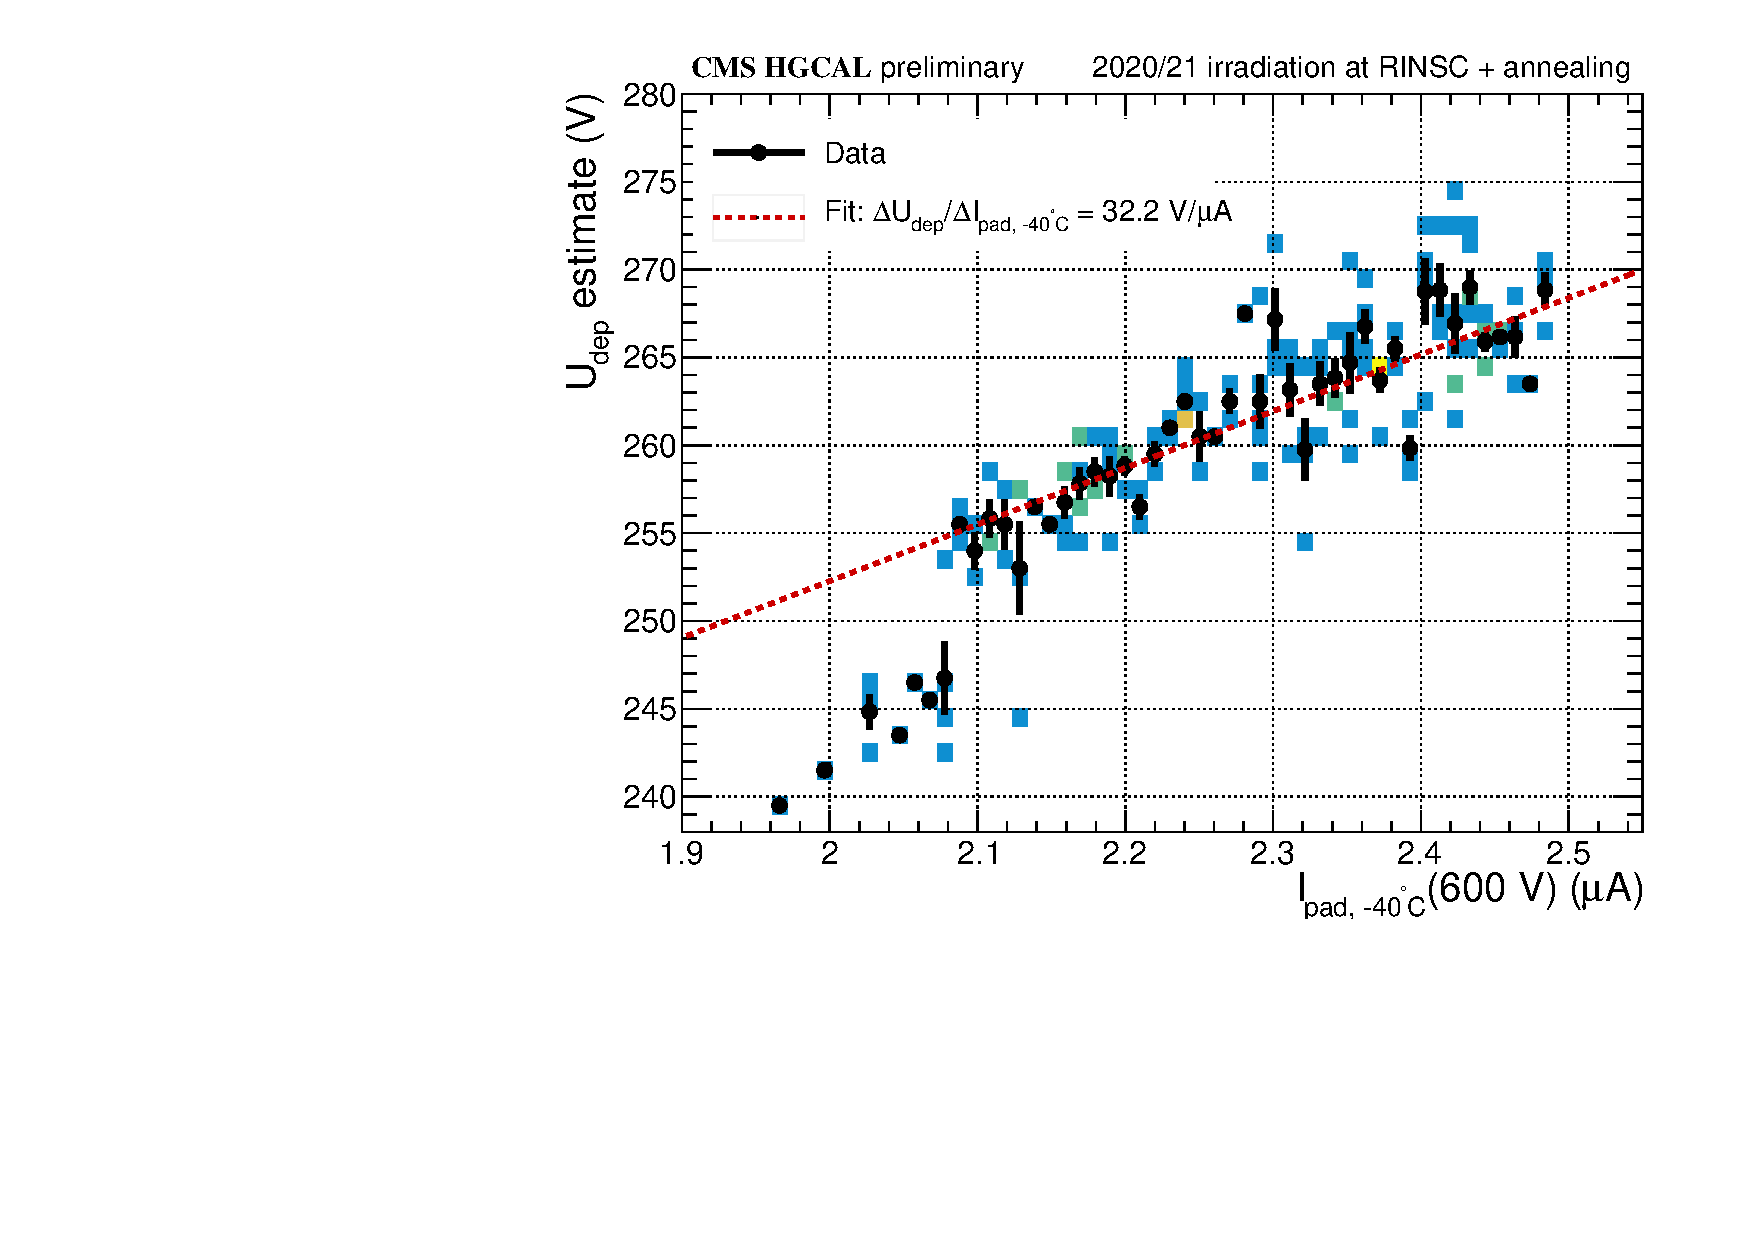
\includegraphics[width=0.999\textwidth]{plots/Vdep_vs_fluence/Vdep_vs_current_5414.pdf}
		\subcaption{
			}
			\label{plot:Vdep_vs_current_5414}
	\end{subfigure}
	\caption{
		(a) Per-pad depletion voltage estimates for a \SI{200}{\micron} LD example sensor irradiated to 1.9E+15$~\neqcm$, and 
		(b) their correlation to the per-pad leakage current, interpretable as proxy for the fluence.
	}
\end{figure}
We find that the per-pad capacitance after irradiation still scales reasonably well with the area of the pad, cf.~\ref{plot:pad_CV_channels}.
Deviations from this scaling amount to less than \SI{5}{\percent}.
Between full pads, the inter-pad capacitance has been in measured to be \SI{2}{\pico\farad}.
The deviation of up to \SI{5}{\percent} may hint at differing inter-pad capacitances between other pads geometries.
However, further investigation of this hypothesis is beyond the scope of this paper. 
\ref{plot:pad_invCV_sensor} illustrates that the estimated depletion voltages in this work scale primarily with the associated thickness of the depleted zone. 

The profile of estimated depletion voltage of a representative sensor is shown in~\ref{plot:Vdep_hexplot_0541_04}.
Those estimates exhibit positive correlation with the leakage currents, taken as proxy for the fluence, cf. \ref{plot:Vdep_hexplot_0541_04}.
In fact, the obtained correlation coefficient from this analysis is positive for all tested sensors where full depletion could be reached.
This circumstance can be understood as further evidence for the presence of a fluence profile inside the beam port during irradiation.

\subsection{Discussion}
\label{subsec:discussion}
The leakage currents measured from the neutron-irradiated silicon sensors in this work exhibit both qualitative and quantitative consistency with previous R$\&$D on irradiated silicon sensors, and in particular they are found to be independent on the silicon fabrication process.
Furthermore, unchanged end-capacitances and reduced depletion voltages after beneficial annealing are qualitatively consistent with previous R$\&$D.
The accurate determination of depletion voltages of irradiated silicon sensors is delicate and requires a thorough understanding of the underlying circuitry, in particular a dedicated choice of f$_\text{LCR}$ and of R$_\text{bias}$ on the switch card, and are biased by the choice of tested bias voltages.
At this point, we therefore refrain from more quantitative statements on the depletion voltages and their variations between different sensor fabrication parameters.\newline
Despite this limitation, our findings are in full support of the radiation-hardness of the first prototypes of 8'' HGCAL silicon sensors.
By implication, proper operation of the RINSC neutron-irradiation facility for the irradiation of 8'' silicon sensors could be demonstrated for the first time.
However, more accurate studies on the electrical sensor properties after neutron-irradiation would need to incorporate the systematic uncertainty on the effective annealing during irradiation, that is due to the temperature evolution and its potential lateral profile inside the reactor's beam port.
Similarly, an accurate assessment of the actual fluence at each pad would have to address the neutron flux profile, for whose existence this work provides first evidence.